\documentclass{beamer}


\usetheme[progressbar=frametitle]{metropolis}
\usepackage{appendixnumberbeamer}

\usepackage{booktabs}
\usepackage[scale=2]{ccicons}

%\usepackage{pgfplots}
%\usepgfplotslibrary{dateplot}

\usepackage{xspace}
\newcommand{\themename}{\textbf{\textsc{metropolis}}\xspace}

%\setbeamertemplate{footline} % To remove the footer line in all slides uncomment this line
%\setbeamertemplate{footline}[page number] % To replace the footer line in all slides with a simple slide count uncomment this line

%\setbeamertemplate{navigation symbols}{} % To remove the navigation symbols from the bottom of all slides uncomment this line


\usepackage{graphicx} % Allows including images
\usepackage{grffile}
\usepackage{amsmath}
\usepackage{adjustbox} 
% have to have Mozilla's=Fira Sans} font and XeTeX installed to use full typography.

%----------------------------------------------------------------------------------------
%	TITLE PAGE
%----------------------------------------------------------------------------------------

\title{Alliance Participation and Military Spending}
\date{January 27, 2019}
\author{Joshua Alley}
\institute{Texas A\&M University}


\begin{document}

 \maketitle


%----------------------------------------------------------------------------------------
%	PRESENTATION SLIDES
%----------------------------------------------------------------------------------------


%------------------------------------------------
% Here's my point. 
 \begin{frame}[standout]

Whether alliance treaty participation increases or decreases military spending depends on alliance treaty strength and state capability. 

 \end{frame}

%------------------------------------------------
% The two subpoints 
 \begin{frame}[standout]

\setbeamercovered{invisible}

\uncover<1>{1: Strong alliance treaties decrease growth in military spending from alliance participation for major powers.} 

\uncover<2>{2: Strong alliance treaties increase growth in military spending from alliance participation for non-major powers.}

 \end{frame}


%------------------------------------------------

\begin{frame}{Scholarly Importance: Competing Expectations and Results}

\textit{Expectations}: \uncover<2->{Force Multiplier} \uncover<3->{or Foreign Entanglement?}

\uncover<4->{
\begin{table}[hbt!]
\begin{center}
\begin{tabular}{lccc}
     & Decrease & Increase & Null \\
\hline
Most \& Siverson 1987  &  &  & X \\
Conybeare 1994 & X & &  \\
Diehl 1994 &  & X &  \\
Goldsmith 2003 &  &  & X \\
Morgan \& Palmer 2006 &  & X & \\ 
Quiroz-Flores 2011 &  & X &  \\ 
Digiuseppe \& Poast 2016 & X &  & \\ 
Horowitz et al 2017 &  & X & \\ 
\hline
\end{tabular}
\end{center} 
\end{table}
}

 \end{frame}


%------------------------------------------------

\begin{frame}{Alliance Heterogeneity}

\begin{figure}
	\centering
		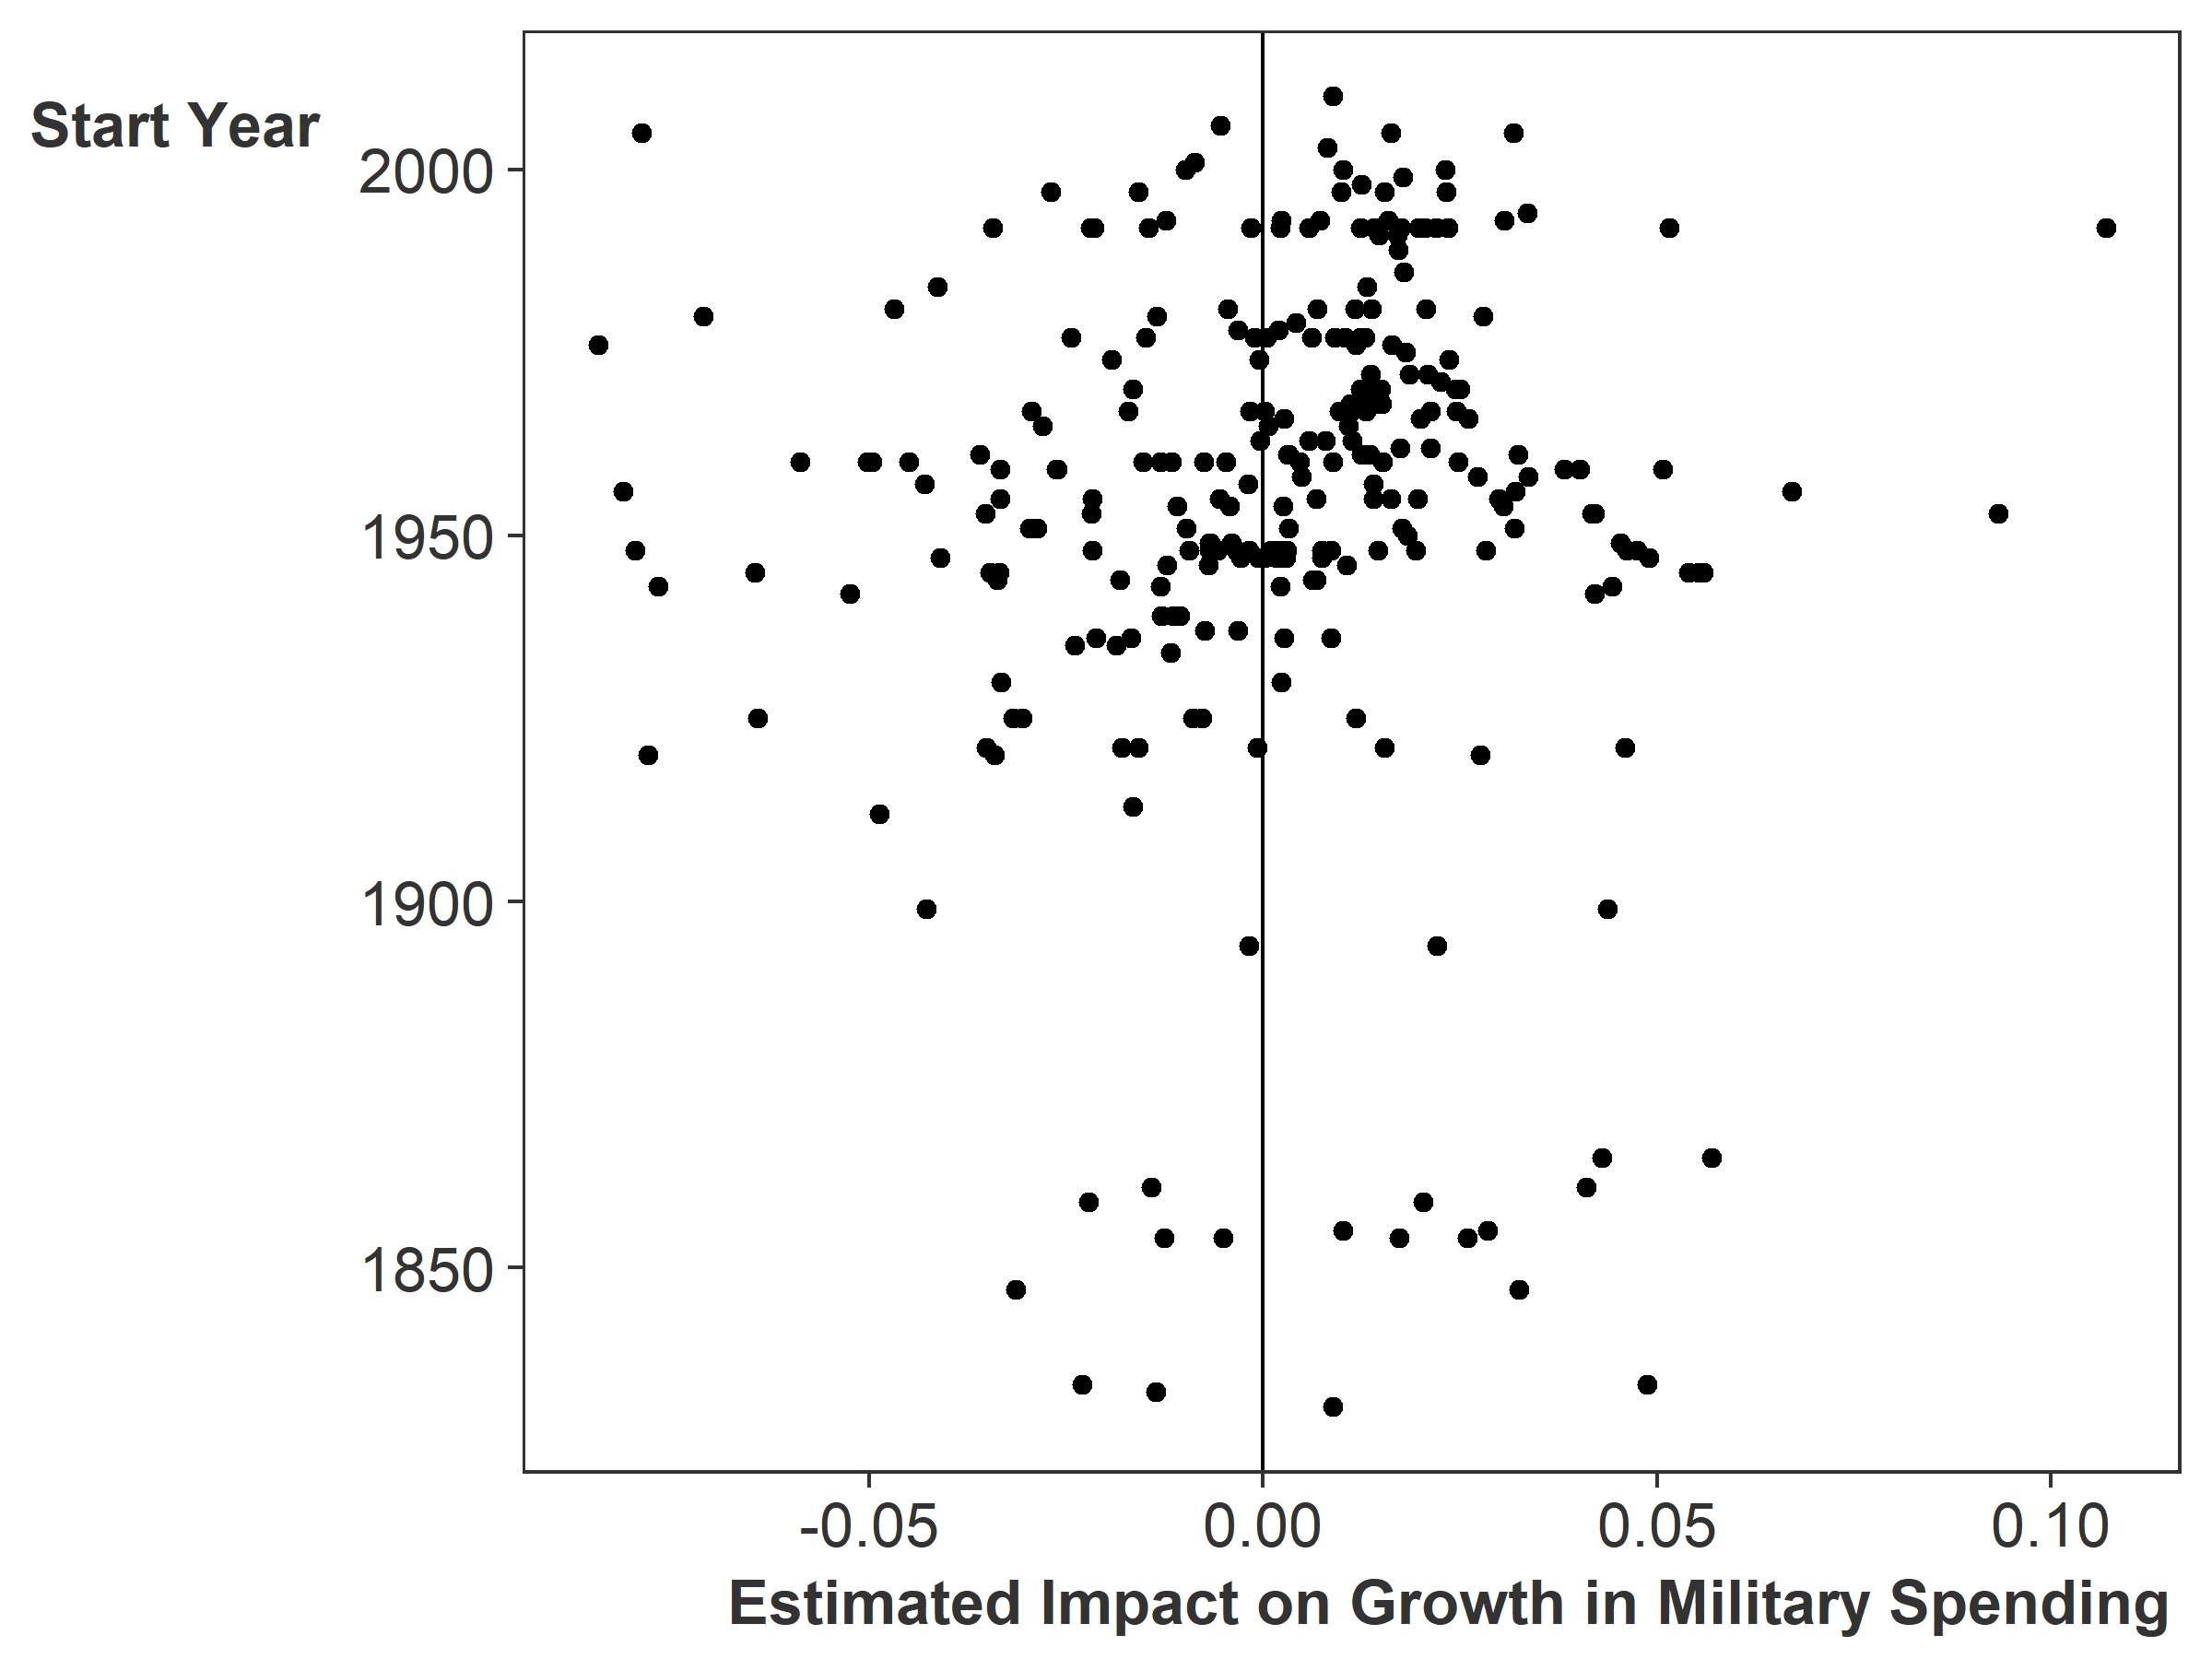
\includegraphics[width=0.95\textwidth]{lambda-est-full.png}
	\label{fig:lambda-est-full}
\end{figure}


 \end{frame}


%------------------------------------------------

\begin{frame}{Relevance}

\begin{figure}[htbp]
	\centering
		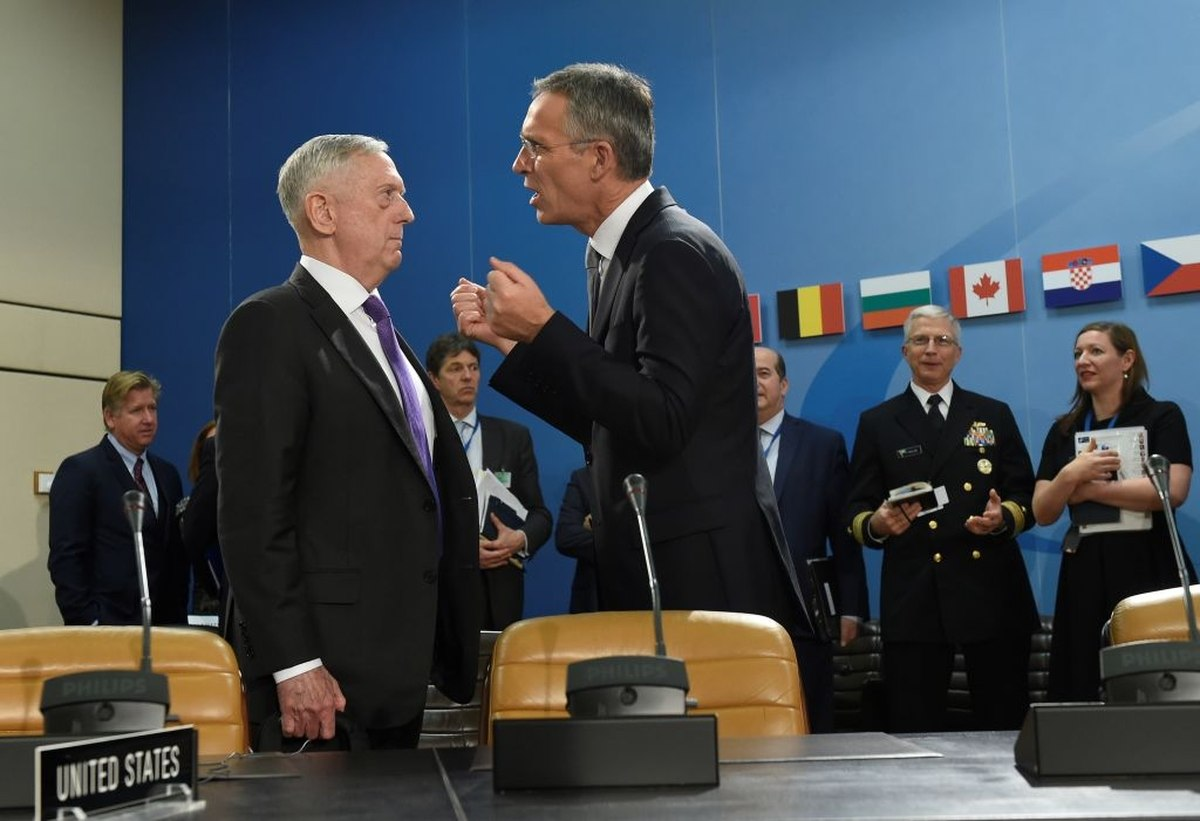
\includegraphics[width=0.95\textwidth]{mattis-nato.jpg}
	\label{fig:mattis-nato}
\end{figure}


\end{frame}

%------------------------------------------------

\begin{frame}{Outline}

I make my claim about alliance participation and military spending in two ways: 

\pause
\begin{enumerate}
\item Argument: Treaty Strength and State Capability
\pause
\item Statistical Analysis 
\end{enumerate}


\end{frame}

%------------------------------------------------

\section{Argument}

%------------------------------------------------

%\begin{frame}{Assumptions}

%\begin{itemize} 
%\item Military spending has opportunity costs, which decrease with greater state size. 
%\pause 
%\item Alliances are a costly signal of shared foreign policy interests: credible commitment to intervene.  
%\end{itemize}


%\end{frame}

%------------------------------------------------

\begin{frame}{Formal Treaty Strength}

Not all alliances are equally deep and costly. Strength depends on costs an ally incurs or would incur. 

\begin{itemize} 
\pause
\item Potential Costs: honoring or breaking promises of support.
\pause
\item Sunk costs promises: commitment to take costly action. 
\pause
\item Strong/deep formal commitments increase foreign policy gains from alliance participation. 
\pause 
\item But the same hands tying limits freedom of action for members. 
\end{itemize}  


\end{frame}


%------------------------------------------------

\begin{frame}{State Capability}

\setbeamercovered{invisible} 

\begin{columns}

% Major powers
\begin{column}{0.5\textwidth}
\textbf{Major Powers}

\begin{itemize}
\uncover<2->{\item Alliances \& Spending: External Influence}
\uncover<3->{\item $\mbox{Influence} = \mbox{Probability Intervention} \times \mbox{Capability}$}
\uncover<4->{\item Strong treaties $\uparrow$ influence without $\uparrow$ spending} 
\end{itemize} 
\end{column}



\begin{column}{0.5\textwidth}
\textbf{Non-Major Powers}

\begin{itemize}
\uncover<5->{\item Alliances \& Spending: Territorial Security}\
\uncover<6->{\item Replace domestic expenditure with allied capability.}
\uncover<7->{\item Strong treaties restrict freedom of action: alliance value and allied influence.} 
\end{itemize} 

\end{column}
\end{columns}

\end{frame}



%------------------------------------------------

\begin{frame}[standout]


\begin{quote}
\textsc{Hypothesis 1}: As alliance treaty strength increases, growth in major power military spending from alliance participation will decrease. 
\end{quote} 
\pause 
\begin{quote}
\textsc{Hypothesis 2}: As alliance treaty strength increases, growth in non-major power military spending from alliance participation will increase. 
\end{quote} 


\end{frame}



%------------------------------------------------

\section{Empirical Analysis} 

%-----------------------------------------------

\begin{frame}{Research Design}

To test these predictions, I need two things: 

\pause 
\begin{enumerate} 
\item Measure of treaty strength--- Measurement Model. 
\pause
\item Connect alliance-level variation with state-level outcomes--- Multilevel Analysis.  
\end{enumerate} 


\end{frame}

%------------------------------------------------

\begin{frame}{Measuring Treaty Strength}

I use a latent variable model (semiparametric mixed factor analysis) to infer formal treaty strength from observed promises. 

\pause 

For each alliance, the posterior mean of the latent factor is my measure of strength. 

%\pause 
%\begin{itemize}
%\item Multiple observed indicators of strength (ATOP): 
%\begin{itemize} 
%\item \textit{Potential costs}: offense, defense, neutrality, consultation, non-aggression, unconditional military support.
%\item \textit{Sunk costs}: bases, integrated command, economic/military aid, IO formation, conclude multiple other agreements. 
%\end{itemize} 
%\pause 
%\item Semiparametric mixed factor analysis. (Murray et al 2013)
%\pause
%\item Mean of the latent factor for each alliance. 
%\end{itemize} 


\end{frame} 


%------------------------------------------------

\begin{frame}{Empirical Analysis: Multilevel Model}

\begin{itemize} 
\item Link alliance-level variation with state-level outcomes. 
\pause
\item Two connected regressions: alliance and state-level. 
\pause 
\item Alliance characteristics modify the association between alliance membership and spending growth.  
\end{itemize} 

\end{frame} 


%------------------------------------------------

\begin{frame}{ML Model}

\[
\begin{array}{cccccc}
\uncover<2->{ & & & & &\mbox{Alliance} \\
& & & & &    \mbox{Characteristics}  \\
\uncover<3->{& & & & \lambda = & \alpha_{all} + \beta_1 \mbox{Str.} + \textbf{X} \beta \\}
& & & & &    \downarrow  \\}
\mbox{Growth} =     & \mbox{Varying}   & + & \mbox{State}   & + & \mbox{Alliance} \\
\mbox{Mil. Ex.}      & \mbox{Intercepts}&   &  \mbox{Vars.} &   & \mbox{Participation} \\
\uncover<3->{\mbox{y} = & \alpha + \alpha^{st} + \alpha^{yr}   & + & \textbf{W} \gamma  & + & \textbf{Z} \lambda \\}
\end{array}
\]


\end{frame}

%------------------------------------------------

\begin{frame}{Sample and Controls}

\begin{itemize}
\item \textbf{Split Sample}: major and non-major power states--- 1816-2007. Alliances with military support. 
\pause
\item \textbf{DV}: Growth in Military Spending $ = \frac{ \mbox{Change Mil. Expend}_t }{ \mbox{Mil. Expend}_{t-1} }$ 
\pause
\item \textbf{Alliance-Level IV}: Mean Treaty Strength
\pause
\item \textbf{State-Level Controls}: Interstate war, Civil War, Annual MIDs, GDP growth, POLITY, Cold War, Rival military expenditures. 
\pause 
\item \textbf{Alliance-Level Controls}: Share of Democracies, Number of Members, wartime, asymmetric obligations, US member (Cold War), USSR member.

\end{itemize} 


\end{frame}


%------------------------------------------------

\section{Results}

%------------------------------------------------

\begin{frame}{Association Between Treaty Strength and Growth in Military Spending} 

\begin{figure}
	\centering
		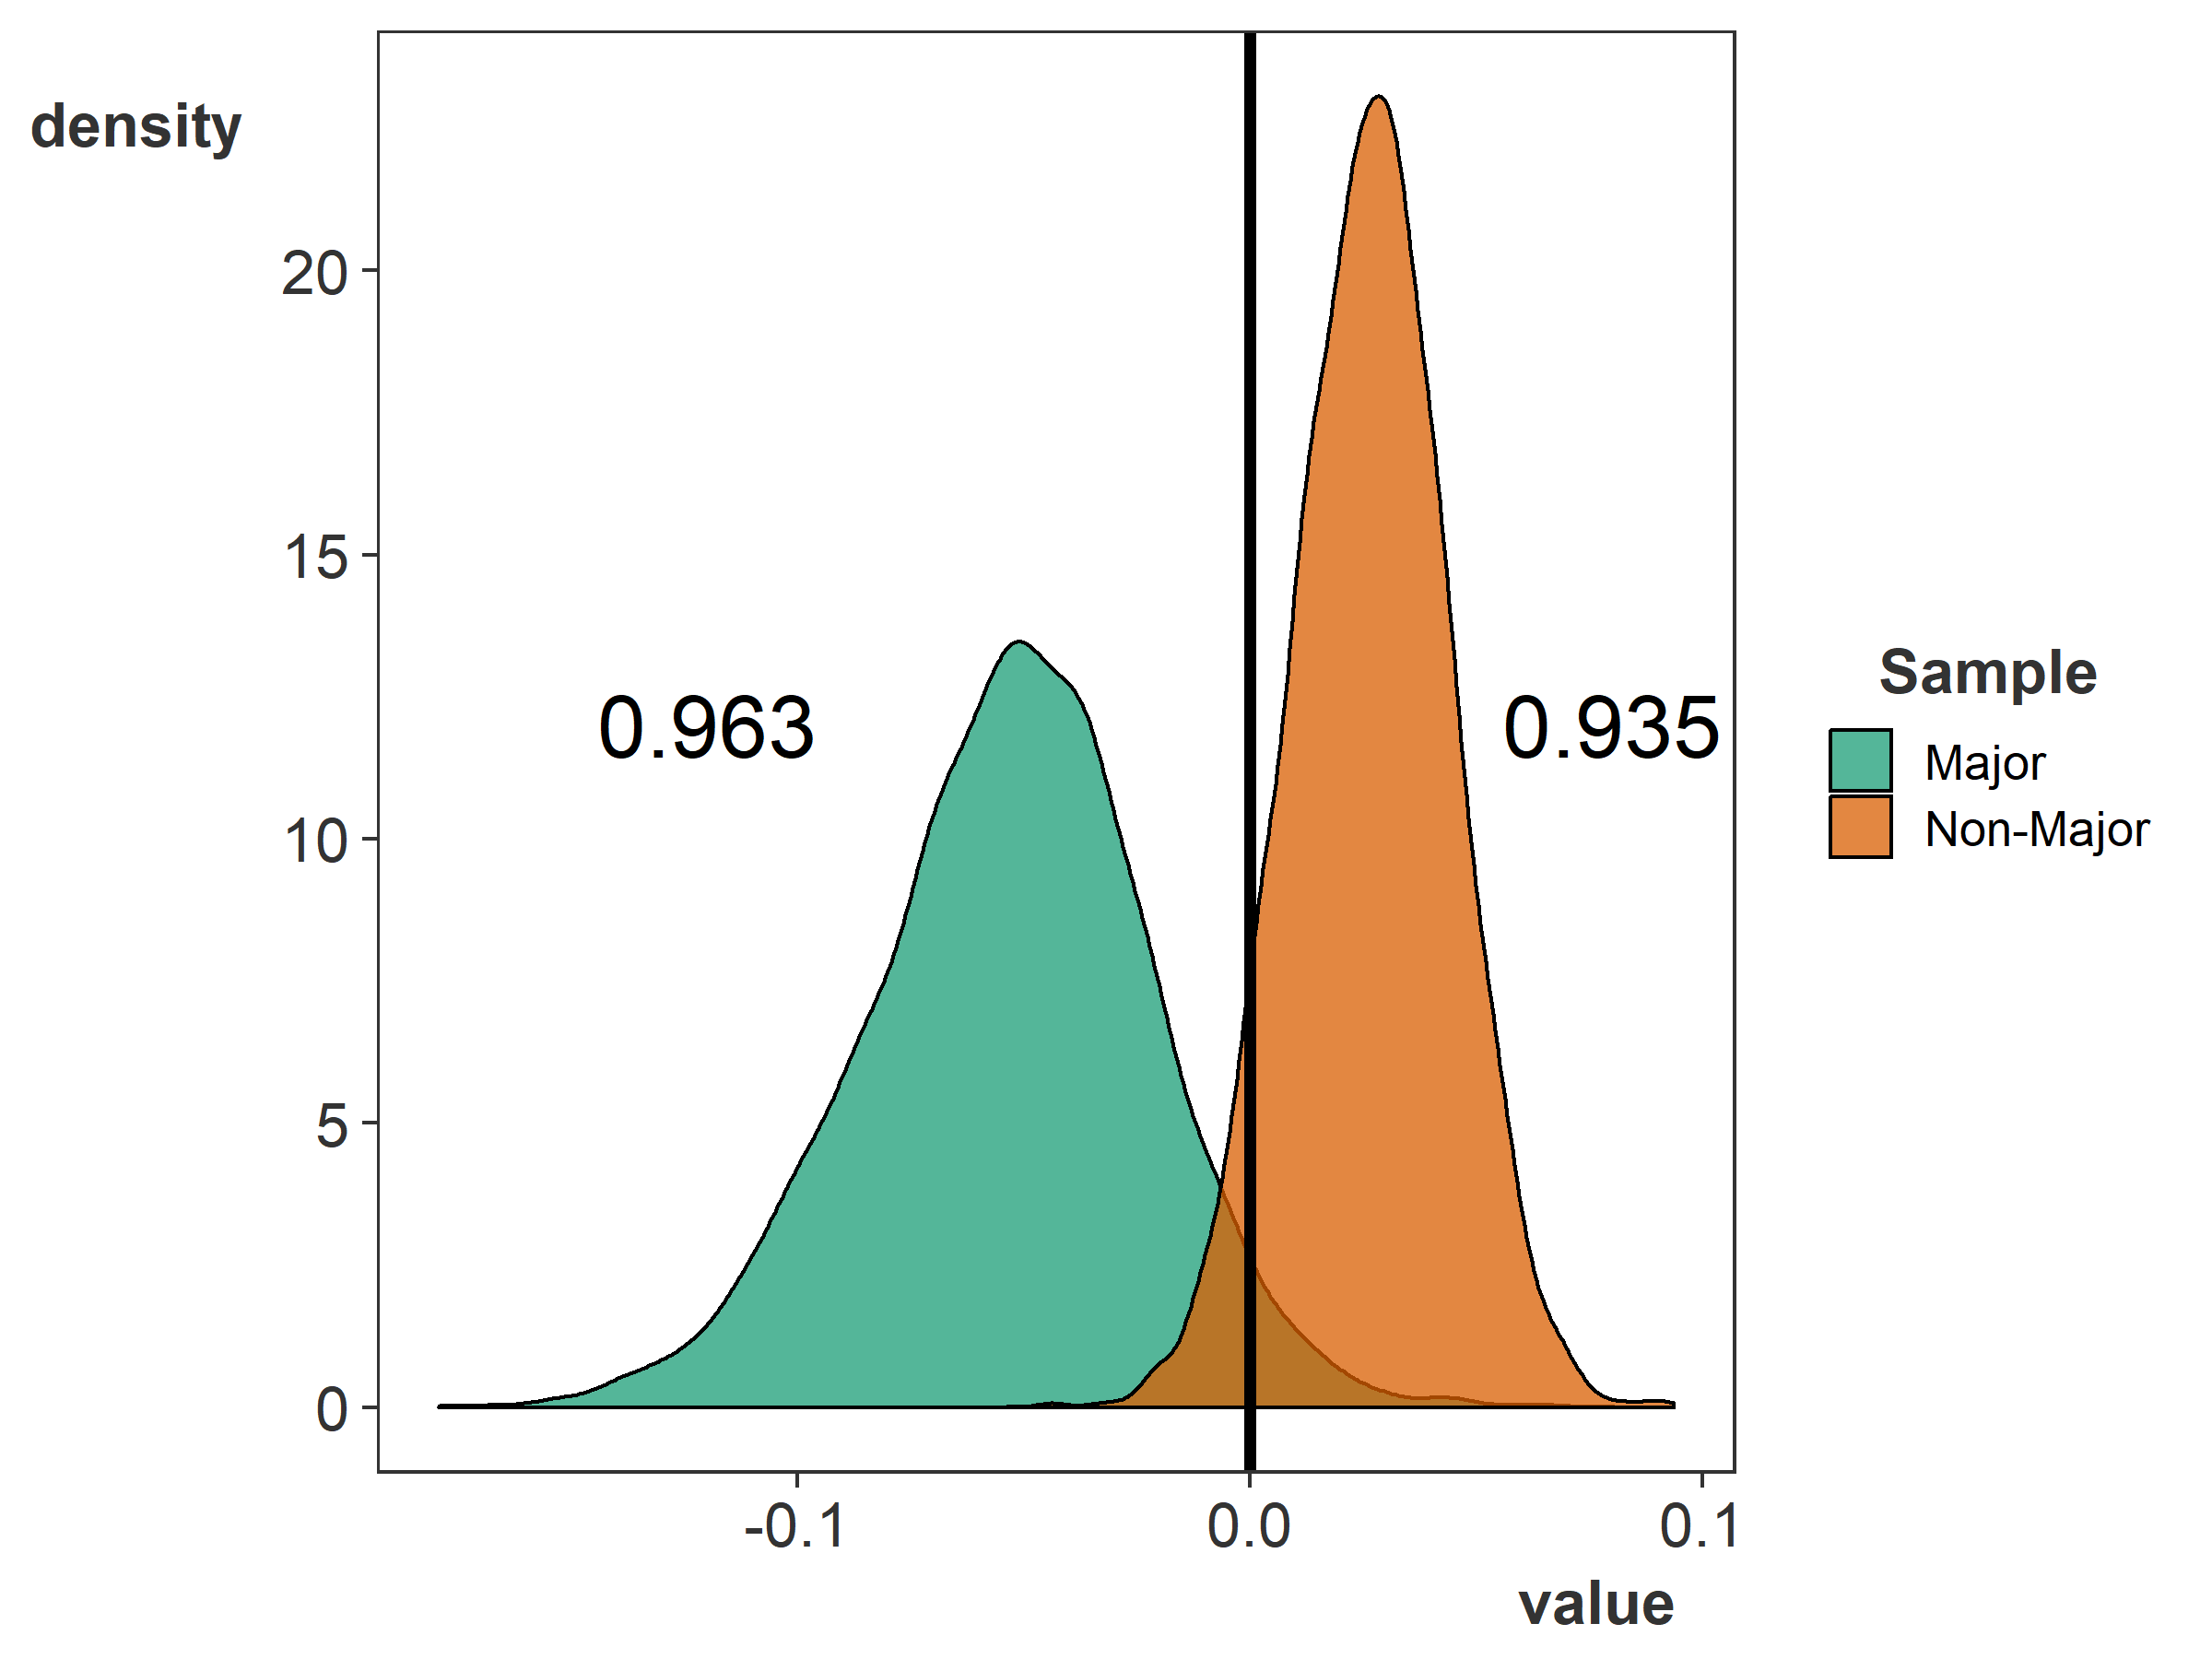
\includegraphics[width=0.95\textwidth]{str-post.png}
	\label{fig:str-post}
\end{figure}


\end{frame}




%-----------------------------------------------

\section{Conclusion}

%-----------------------------------------------

\begin{frame}{Conclusion}

Whether alliance treaty participation increases or decreases military spending depends on state capability and alliance treaty strength.  


\end{frame}

%-----------------------------------------------

% Here's my point. 
 \begin{frame}[standout]

Thank you! 

jkalley14@tamu.edu

 \end{frame}


%-----------------------------------------------

\appendix 


%-----------------------------------------------

\begin{frame}{Limitations}

\begin{enumerate}
\item Domestic political economy of military spending. 
\pause 
\item Measurement error and missing data. 
\pause 
\item Strategic alliance design
\end{enumerate}

\end{frame}

%------------------------------------------------

\begin{frame}[standout]{Importance} 

\begin{tabular}{lcc}
Sample & Posterior Mean & Median Ex. Growth \\
\hline
Major & -0.05 & 0.04 \\
%\pause
Non-major & 0.03 & 0.06  \\
\end{tabular}

%\pause

US spent \$36.0 billion on NATO in 2018, or 5.5\% of the total defense spending. 


\end{frame}

%------------------------------------------------


\begin{frame}{Alliance-Level Regression Table: Major Powers}

930 observations, with 130 alliances. 

\resizebox{.95\textwidth}{!}{
\begin{tabular}{rrrrrrr}
  \hline
 & mean & S.D. & 5\% & 95\% & n\_eff & $\hat{R}$ \\ 
  \hline
Constant & 0.038 & 0.038 & -0.025 & 0.102 & 3380.954 & 1.000 \\ 
  Latent Str. & -0.054 & 0.031 & -0.107 & -0.005 & 3278.923 & 1.000 \\ 
  Number Members & 0.000 & 0.002 & -0.003 & 0.003 & 4000.000 & 0.999 \\ 
  Democratic Membership & -0.009 & 0.033 & -0.065 & 0.042 & 4000.000 & 1.000 \\ 
  Wartime & -0.057 & 0.035 & -0.115 & -0.001 & 4000.000 & 1.001 \\ 
  Asymmetric & 0.053 & 0.035 & 0.001 & 0.115 & 2218.509 & 1.000 \\ 
  US Member & 0.002 & 0.031 & -0.051 & 0.051 & 4000.000 & 1.000 \\ 
  USSR Member & 0.023 & 0.033 & -0.028 & 0.079 & 4000.000 & 1.000 \\ 
  $\sigma$ Alliances & 0.066 & 0.029 & 0.019 & 0.117 & 599.081 & 1.007 \\ 
   \hline
\end{tabular}
}


\end{frame}

%-----------------------------------------------

\begin{frame}{Alliance-Level Regression Table: Non-Major Powers}

8,668 observations and 192 alliances. 

\resizebox{.95\textwidth}{!}{
\begin{tabular}{rrrrrrr}
  \hline
 & mean & sd & 5\% & 95\% & n\_eff & $\hat{R}$ \\ 
  \hline
Constant & -0.018 & 0.018 & -0.047 & 0.012 & 2211.374 & 1.000 \\ 
  Latent Str. & 0.026 & 0.017 & -0.002 & 0.054 & 2191.382 & 1.000 \\ 
  Number Members & 0.000 & 0.001 & -0.001 & 0.001 & 4000.000 & 1.000 \\ 
  Democratic Membership & -0.031 & 0.015 & -0.056 & -0.009 & 3213.621 & 1.000 \\ 
  Wartime & 0.041 & 0.023 & 0.002 & 0.078 & 4000.000 & 1.000 \\ 
  Asymmetric & -0.031 & 0.021 & -0.065 & 0.003 & 4000.000 & 0.999 \\ 
  US Member & 0.013 & 0.018 & -0.016 & 0.042 & 2895.419 & 1.000 \\ 
  USSR Member & 0.011 & 0.031 & -0.041 & 0.062 & 4000.000 & 1.000 \\ 
  $\sigma$ Alliances & 0.014 & 0.009 & 0.002 & 0.030 & 1254.268 & 1.001 \\ 
   \hline
\end{tabular}
}



\end{frame}


%------------------------------------------------



\begin{frame}{ML Model Specification}

\begin{equation}
y \sim student_t(\mu, \nu, \sigma)
\end{equation}
\begin{equation}
\mu = \alpha + \alpha^{st} + \alpha^{yr} +\textbf{W} \gamma + \textbf{Z} \lambda
\end{equation}

\begin{equation}
\lambda \sim N(\theta, \sigma_{all})
\end{equation} 
\begin{equation}
\theta = \alpha_{all} + \beta_1 \mbox{Treaty Strength} + \textbf{X} \beta
\end{equation}


\end{frame}


%------------------------------------------------

\begin{frame}{Example}

\setbeamercovered{transparent}

\begin{equation*}
\uncover<2->{\mu_{it} =} \uncover<3>{\alpha} \uncover<4>{+ \alpha^{st} + \alpha^{yr}} \uncover<5>{+ W_{it} \gamma} \uncover<6>{+ Z_{it} \lambda}
\end{equation*}

Example year: 

\begin{equation*}
\begin{split}
& \uncover<2->{\mbox{Argentina 1955} = } \uncover<3>{\mbox{Overall mean}} \\
& \uncover<4>{+ \mbox{Argentine Intercept} + \mbox{1955 Intercept}} \\
& \uncover<5>{+ \mbox{Argentine Characteristics}} \\
& \uncover<6>{+ \lambda_{OAS} * \mbox{OAS Expenditure} + \lambda_{Rio} * \mbox{Rio Pact Expenditure}}
\end{split}
\end{equation*}

\uncover<7>{
\begin{equation*}
\lambda_{Rio} = \alpha_{all} + \beta_1 \mbox{Treaty Strength} + \mbox{Controls}
\end{equation*}
} 


\end{frame}


%------------------------------------------------


\begin{frame}[standout]{Z} 

\begin{tabular}{lccc}
State-Year & Rio Pact & Warsaw Pact & \ldots \\
\hline
Argentina 1954 & .347 & 0 & \ldots \\
Argentina 1955 & .418  & 0 & \ldots  \\
 \vdots & \vdots & \vdots & \ldots  
\end{tabular}

 \end{frame}


%------------------------------------------------


\begin{frame}{Priors}

4 Chains with 2,000 samples and 1,000 warmup iterations. 

\begin{table} % Create a table of priors.

 \begin{center}
\begin{tabular}{c} 
$ p(\alpha) \sim N(0, 1)$  \\
$ p(\sigma) \sim \mbox{half-}N(0, 1) $ \\
$ p(\alpha^{yr}) \sim N(0, \sigma^{yr}) $ \\ 
$ p(\sigma^{yr}) \sim N(0, 1) $ \\
$ p(\alpha^{st}) \sim N(0, \sigma^{st}) $ \\ 
$ p(\sigma^{st}) \sim \mbox{half-}N(0, 1) $ \\ 
$ p(\sigma^{all}) \sim \mbox{half-}N(0, 1) $ \\
$ p(\beta) \sim N(0, 1) $ \\
$ p(\gamma) \sim N(0, 1) $ \\ 
$ p(\nu) \sim gamma(2, 0.1)$ 
\end{tabular} 
\end{center} 
\label{tab:priors}
\end{table} 


\end{frame}


%------------------------------------------------


\begin{frame}{Treaty Strength and $\lambda$: Major Powers}

\begin{figure}[htbp]
	\centering
		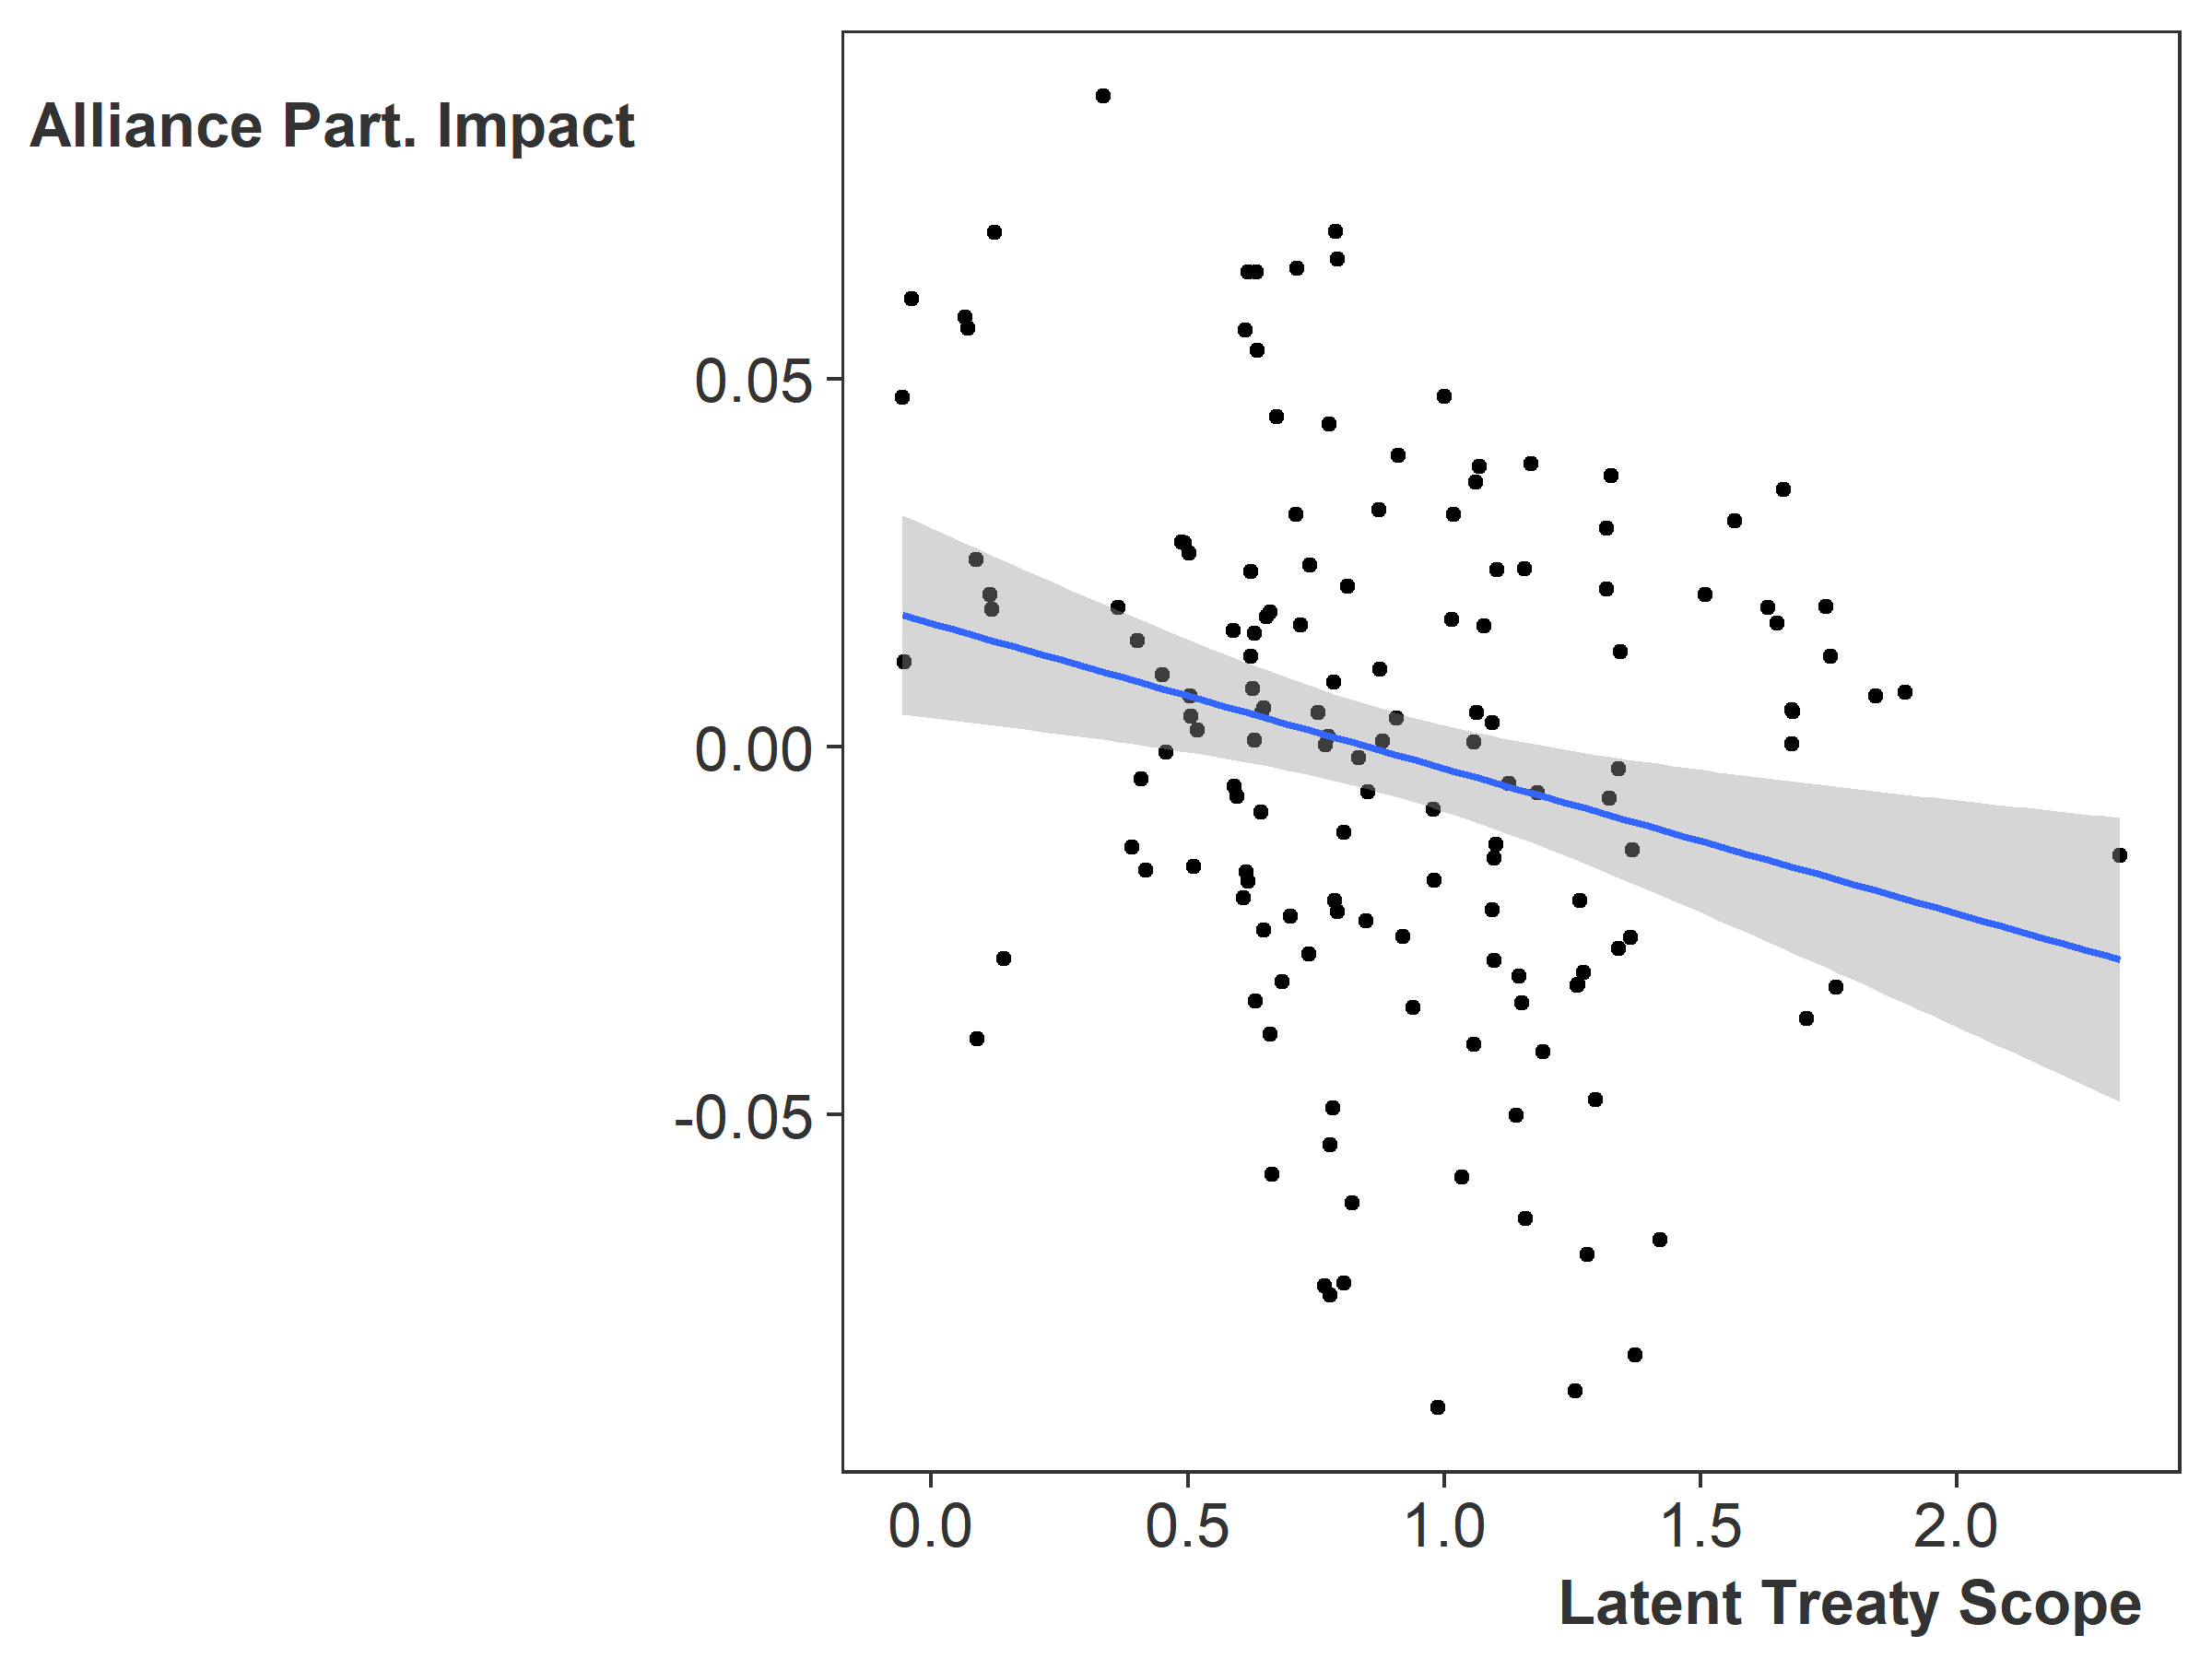
\includegraphics[width=0.95\textwidth]{ls-lambda-maj.png}
	\label{fig:ls-lambda-maj}
\end{figure}



\end{frame}


%------------------------------------------------


\begin{frame}{Treaty Strength and $\lambda$: Non-major Powers}

\begin{figure}
	\centering
		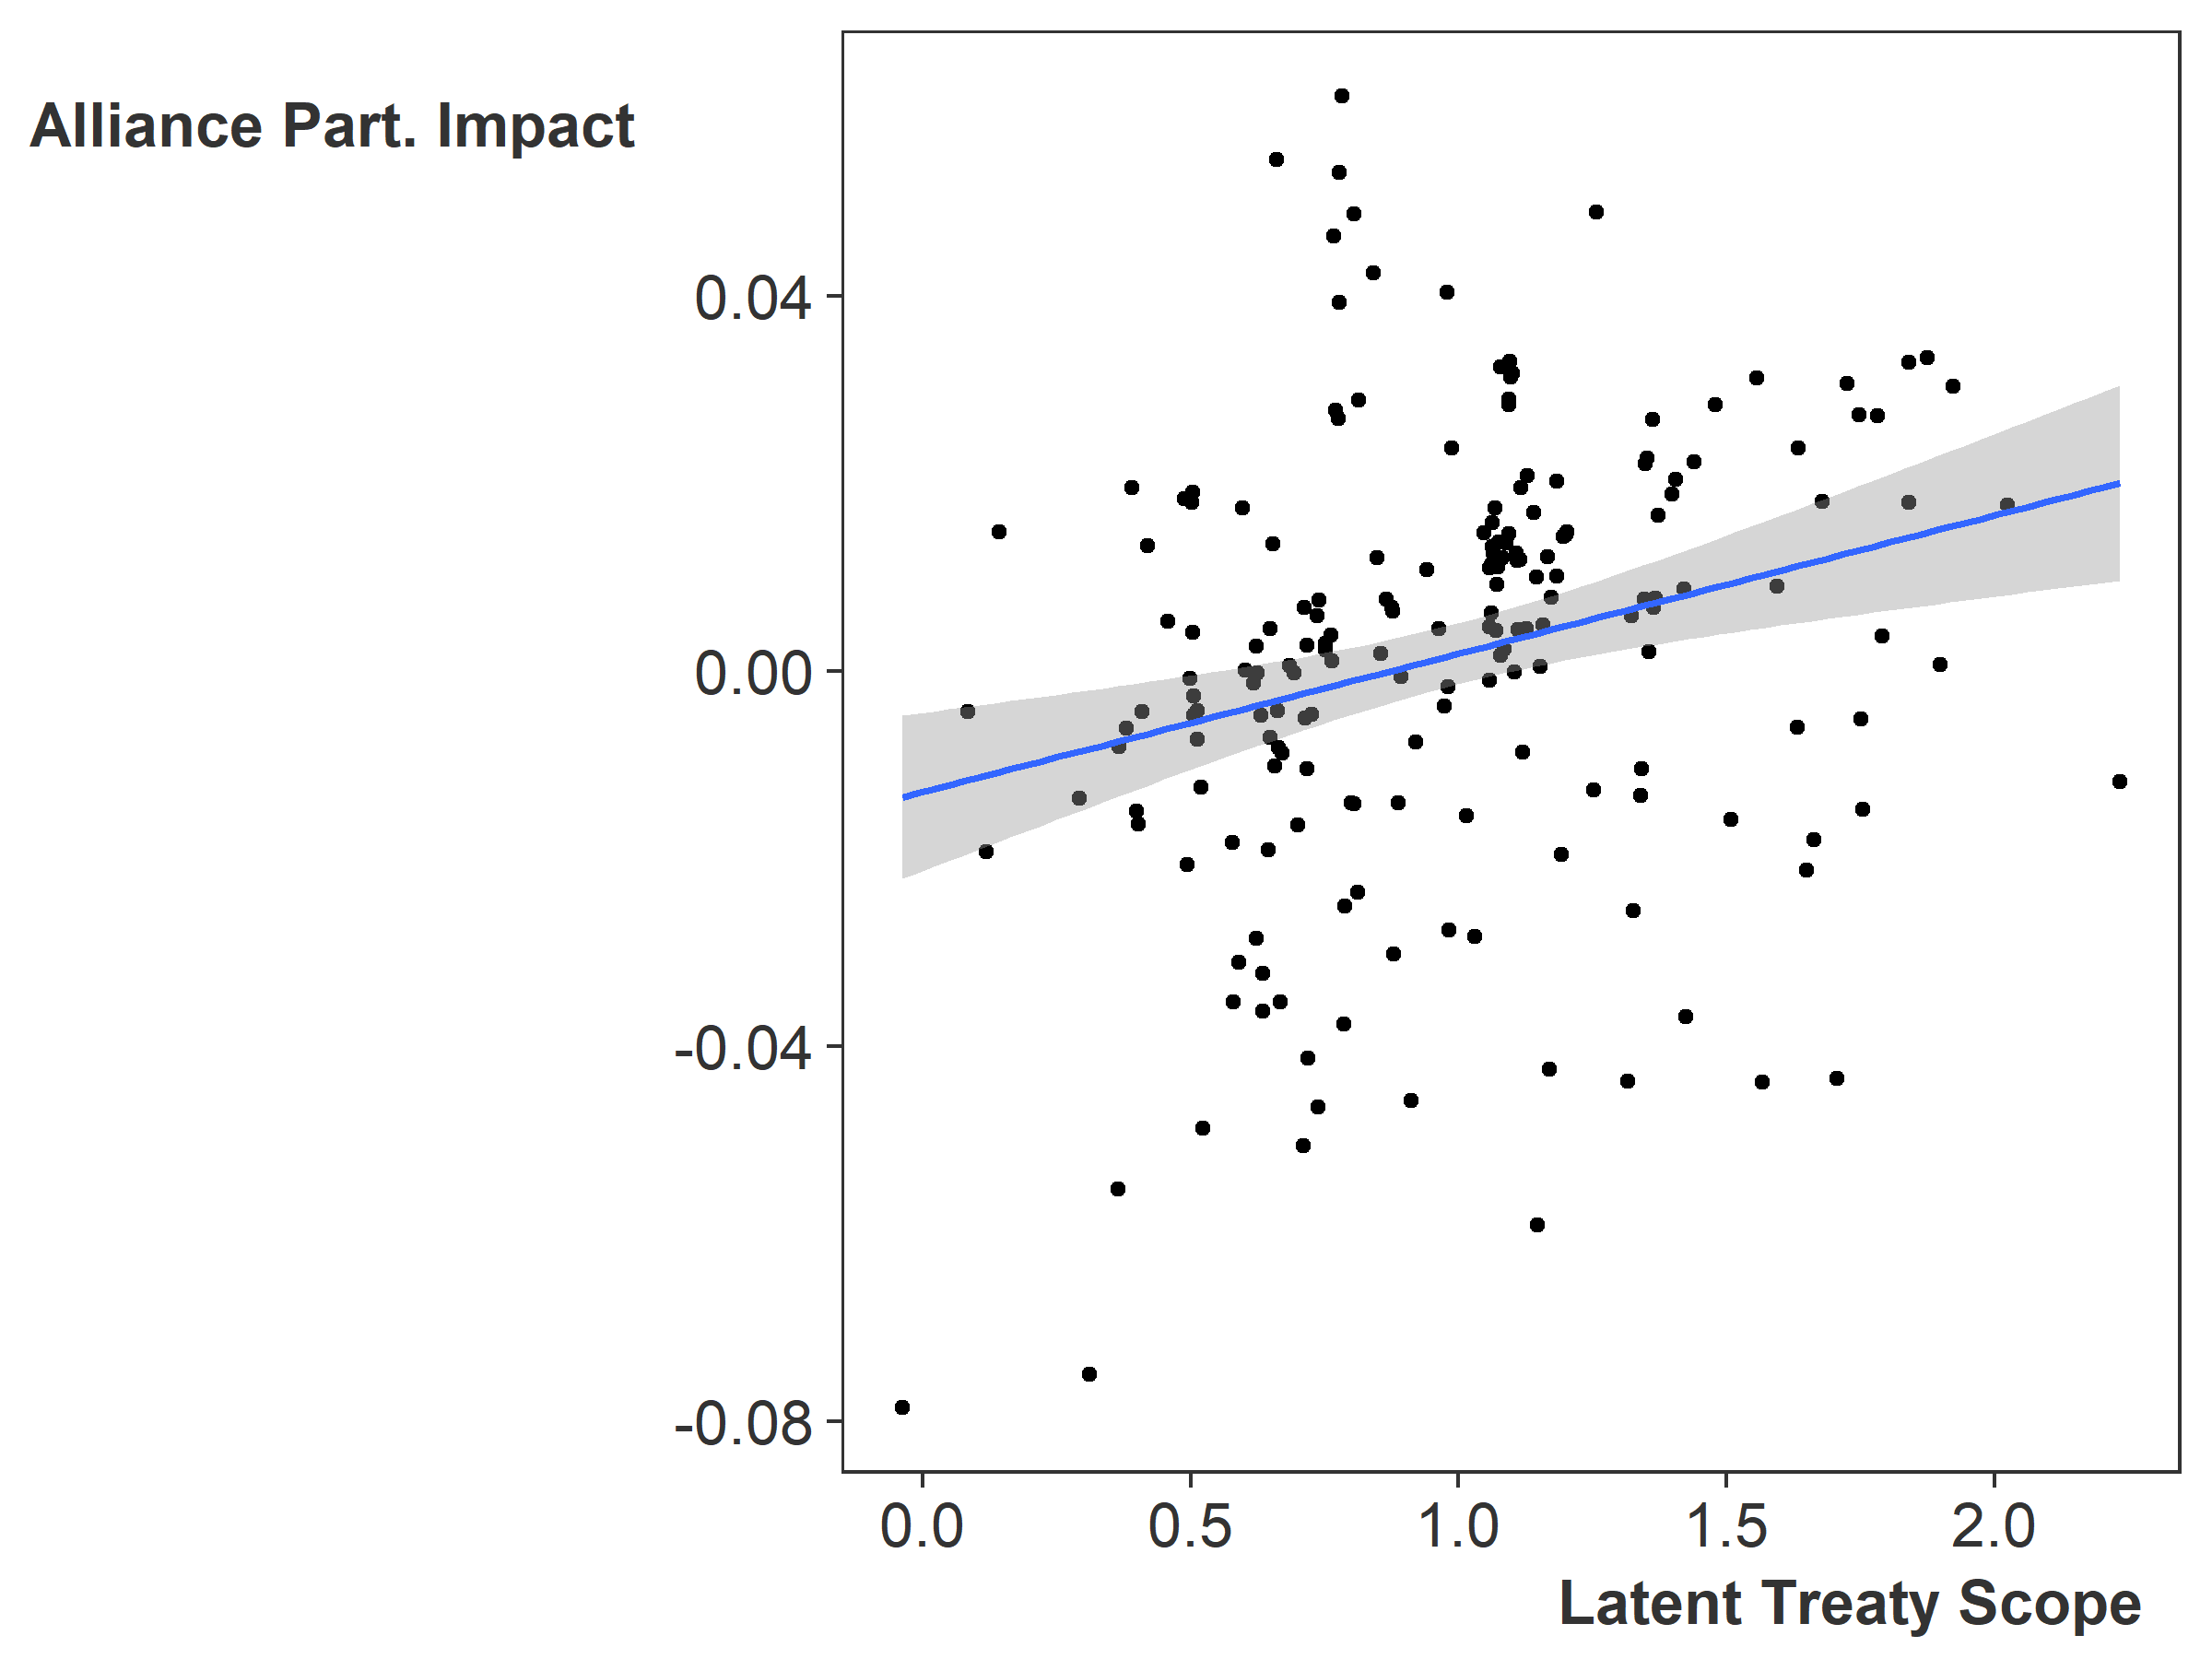
\includegraphics[width=0.95\textwidth]{ls-lambda-min.png}
	\label{fig:ls-lambda-min}
\end{figure}



\end{frame}



%------------------------------------------------

\begin{frame}{Details of Measurement Model}

\begin{itemize}
\item Bayesian Gaussian Copula Factor Model: for mixed data. 
\item Uses copulas to break dependence between latent factors and marginal distributions. 
\item Treats marginals as unknown and keeps them free of dependence. 
\item IMH proposal, 10,000 iteration warmup, 20,000 samples, thinned every 20 draws. 
\item Generalized double Pareto prior for the factor loading--- flexible generalized Laplace distribution with a spike at zero and heavy tails. 
\end{itemize} 


\end{frame}

%------------------------------------------------

\begin{frame}{Latent Measure of Treaty Strength}

% Visual summary of latent measure
\begin{figure}[htbp]
	\centering
		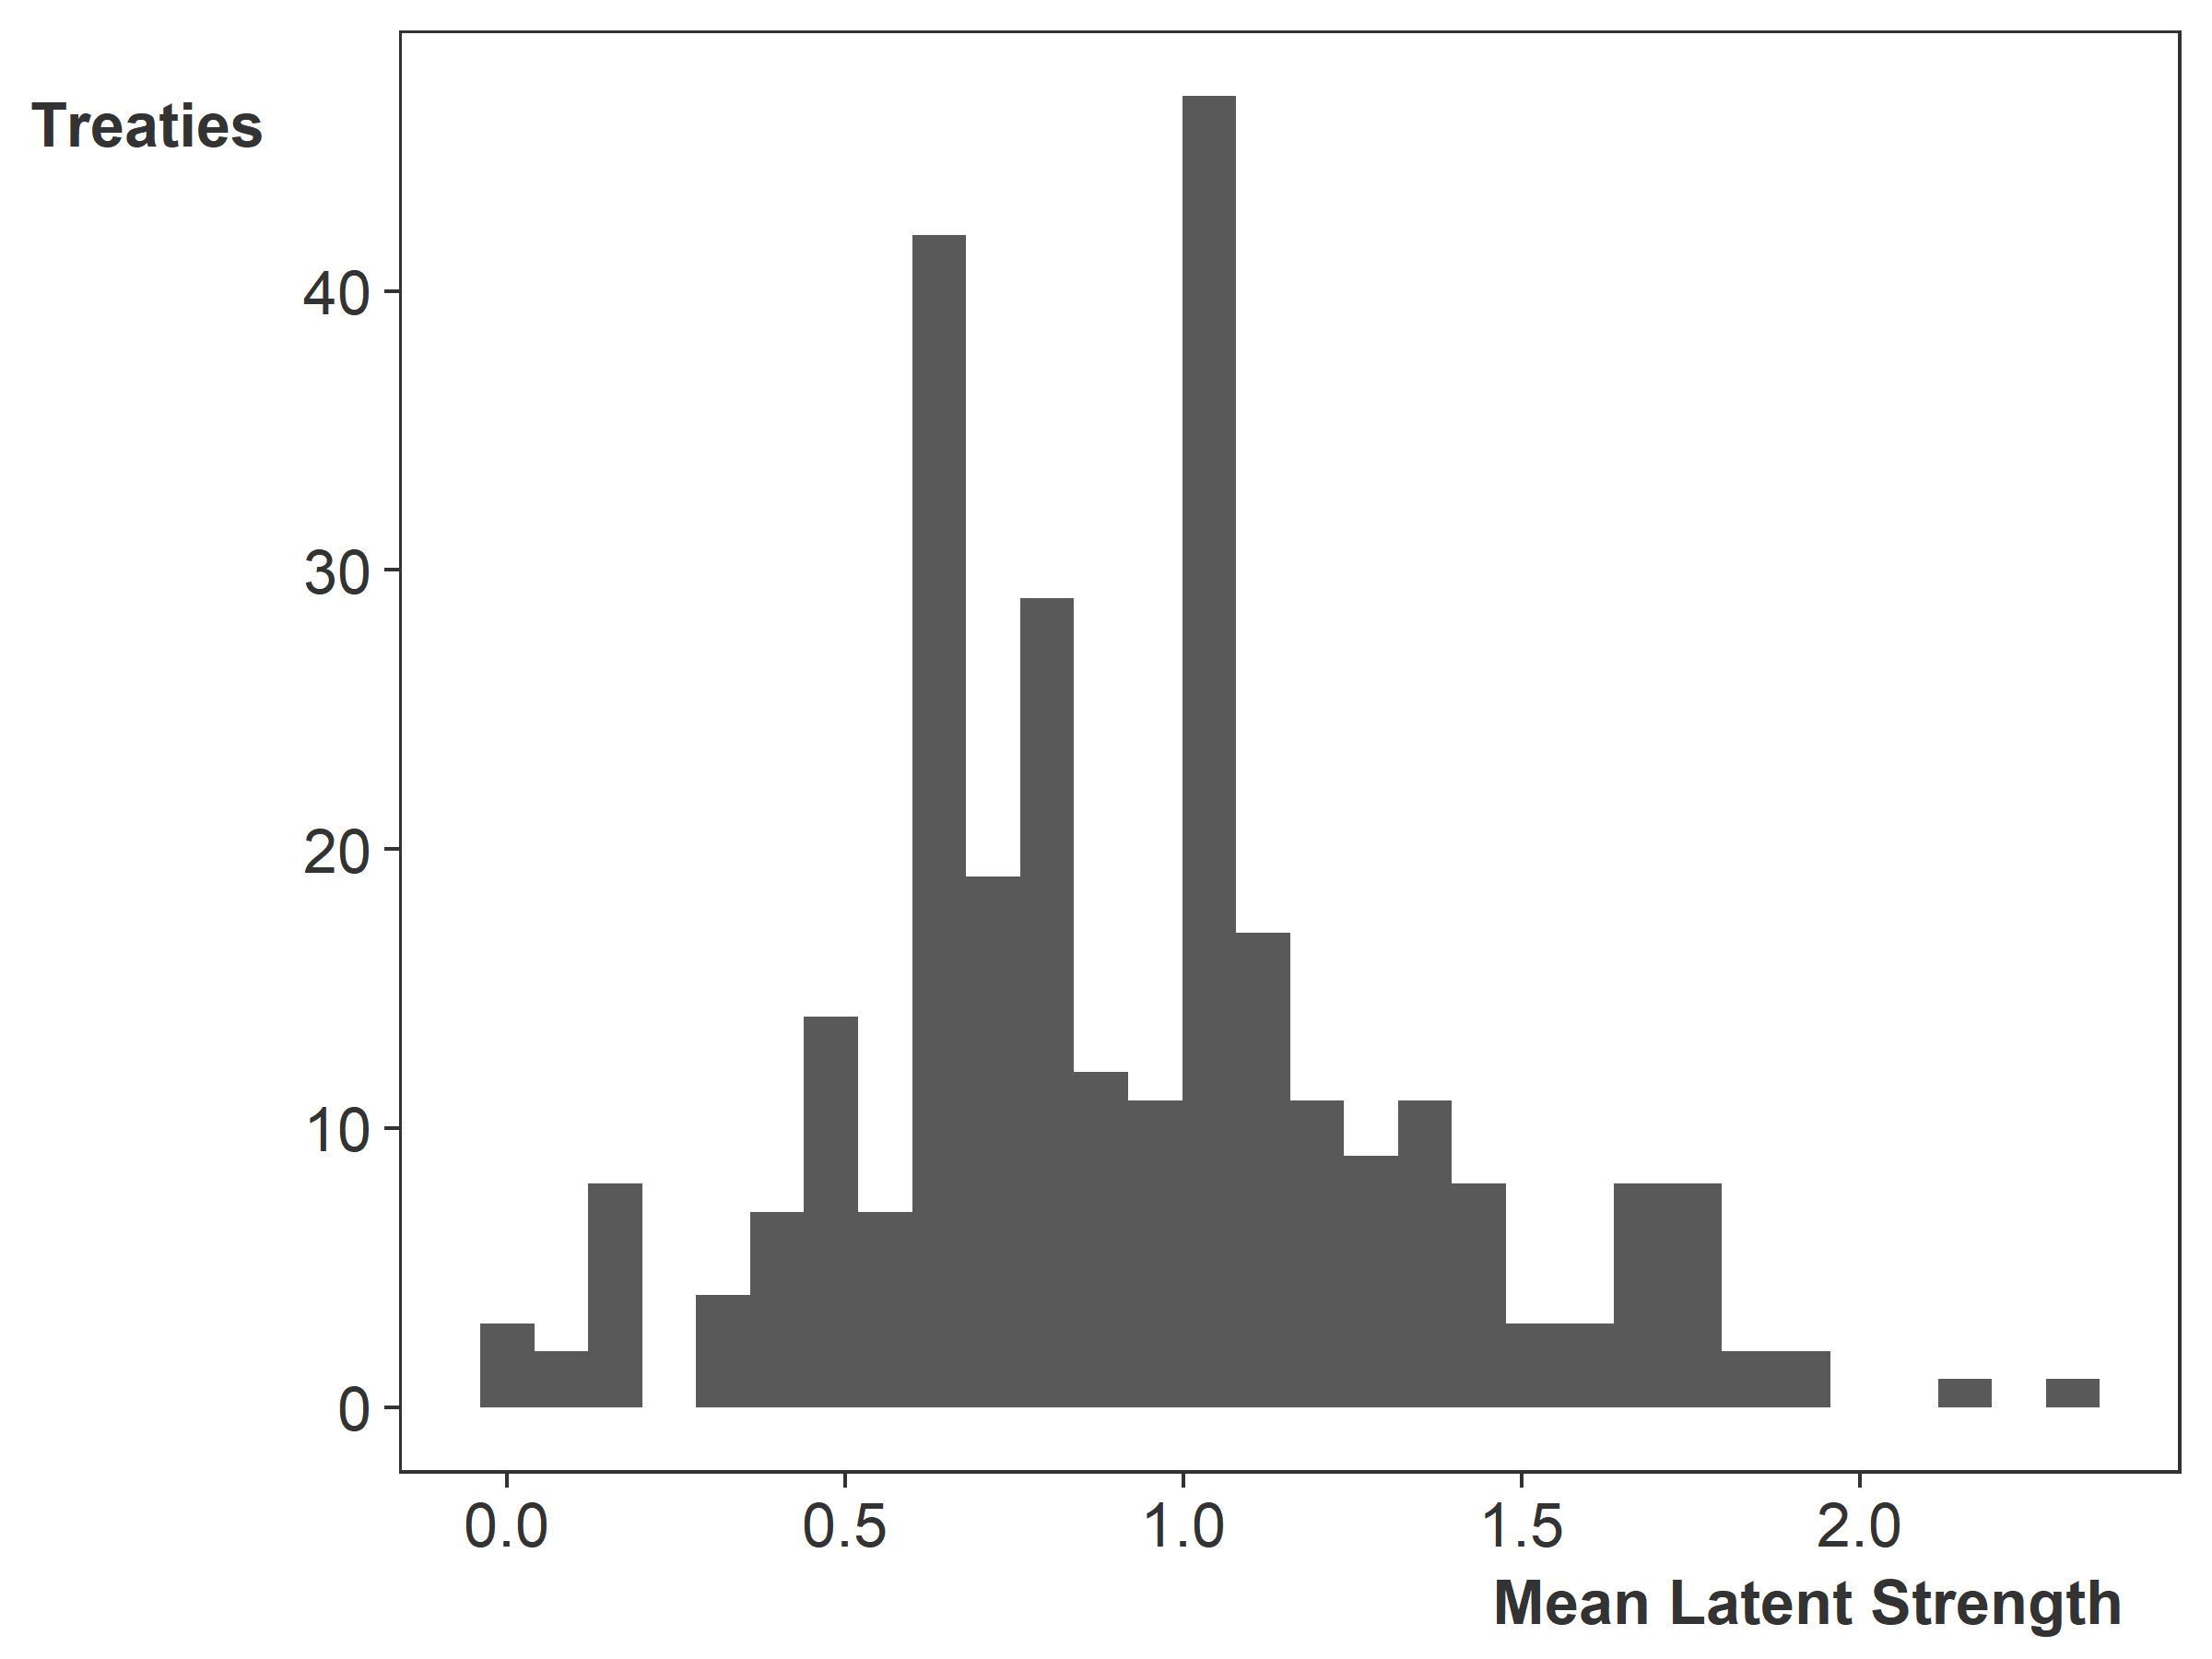
\includegraphics[width=0.95\textwidth]{ls-hist.png}
\end{figure}


\end{frame} 

%------------------------------------------------

\begin{frame}{Latent Measure of Treaty Strength: Weak}

% Visual summary of latent measure
\begin{figure}[htbp]
	\centering
		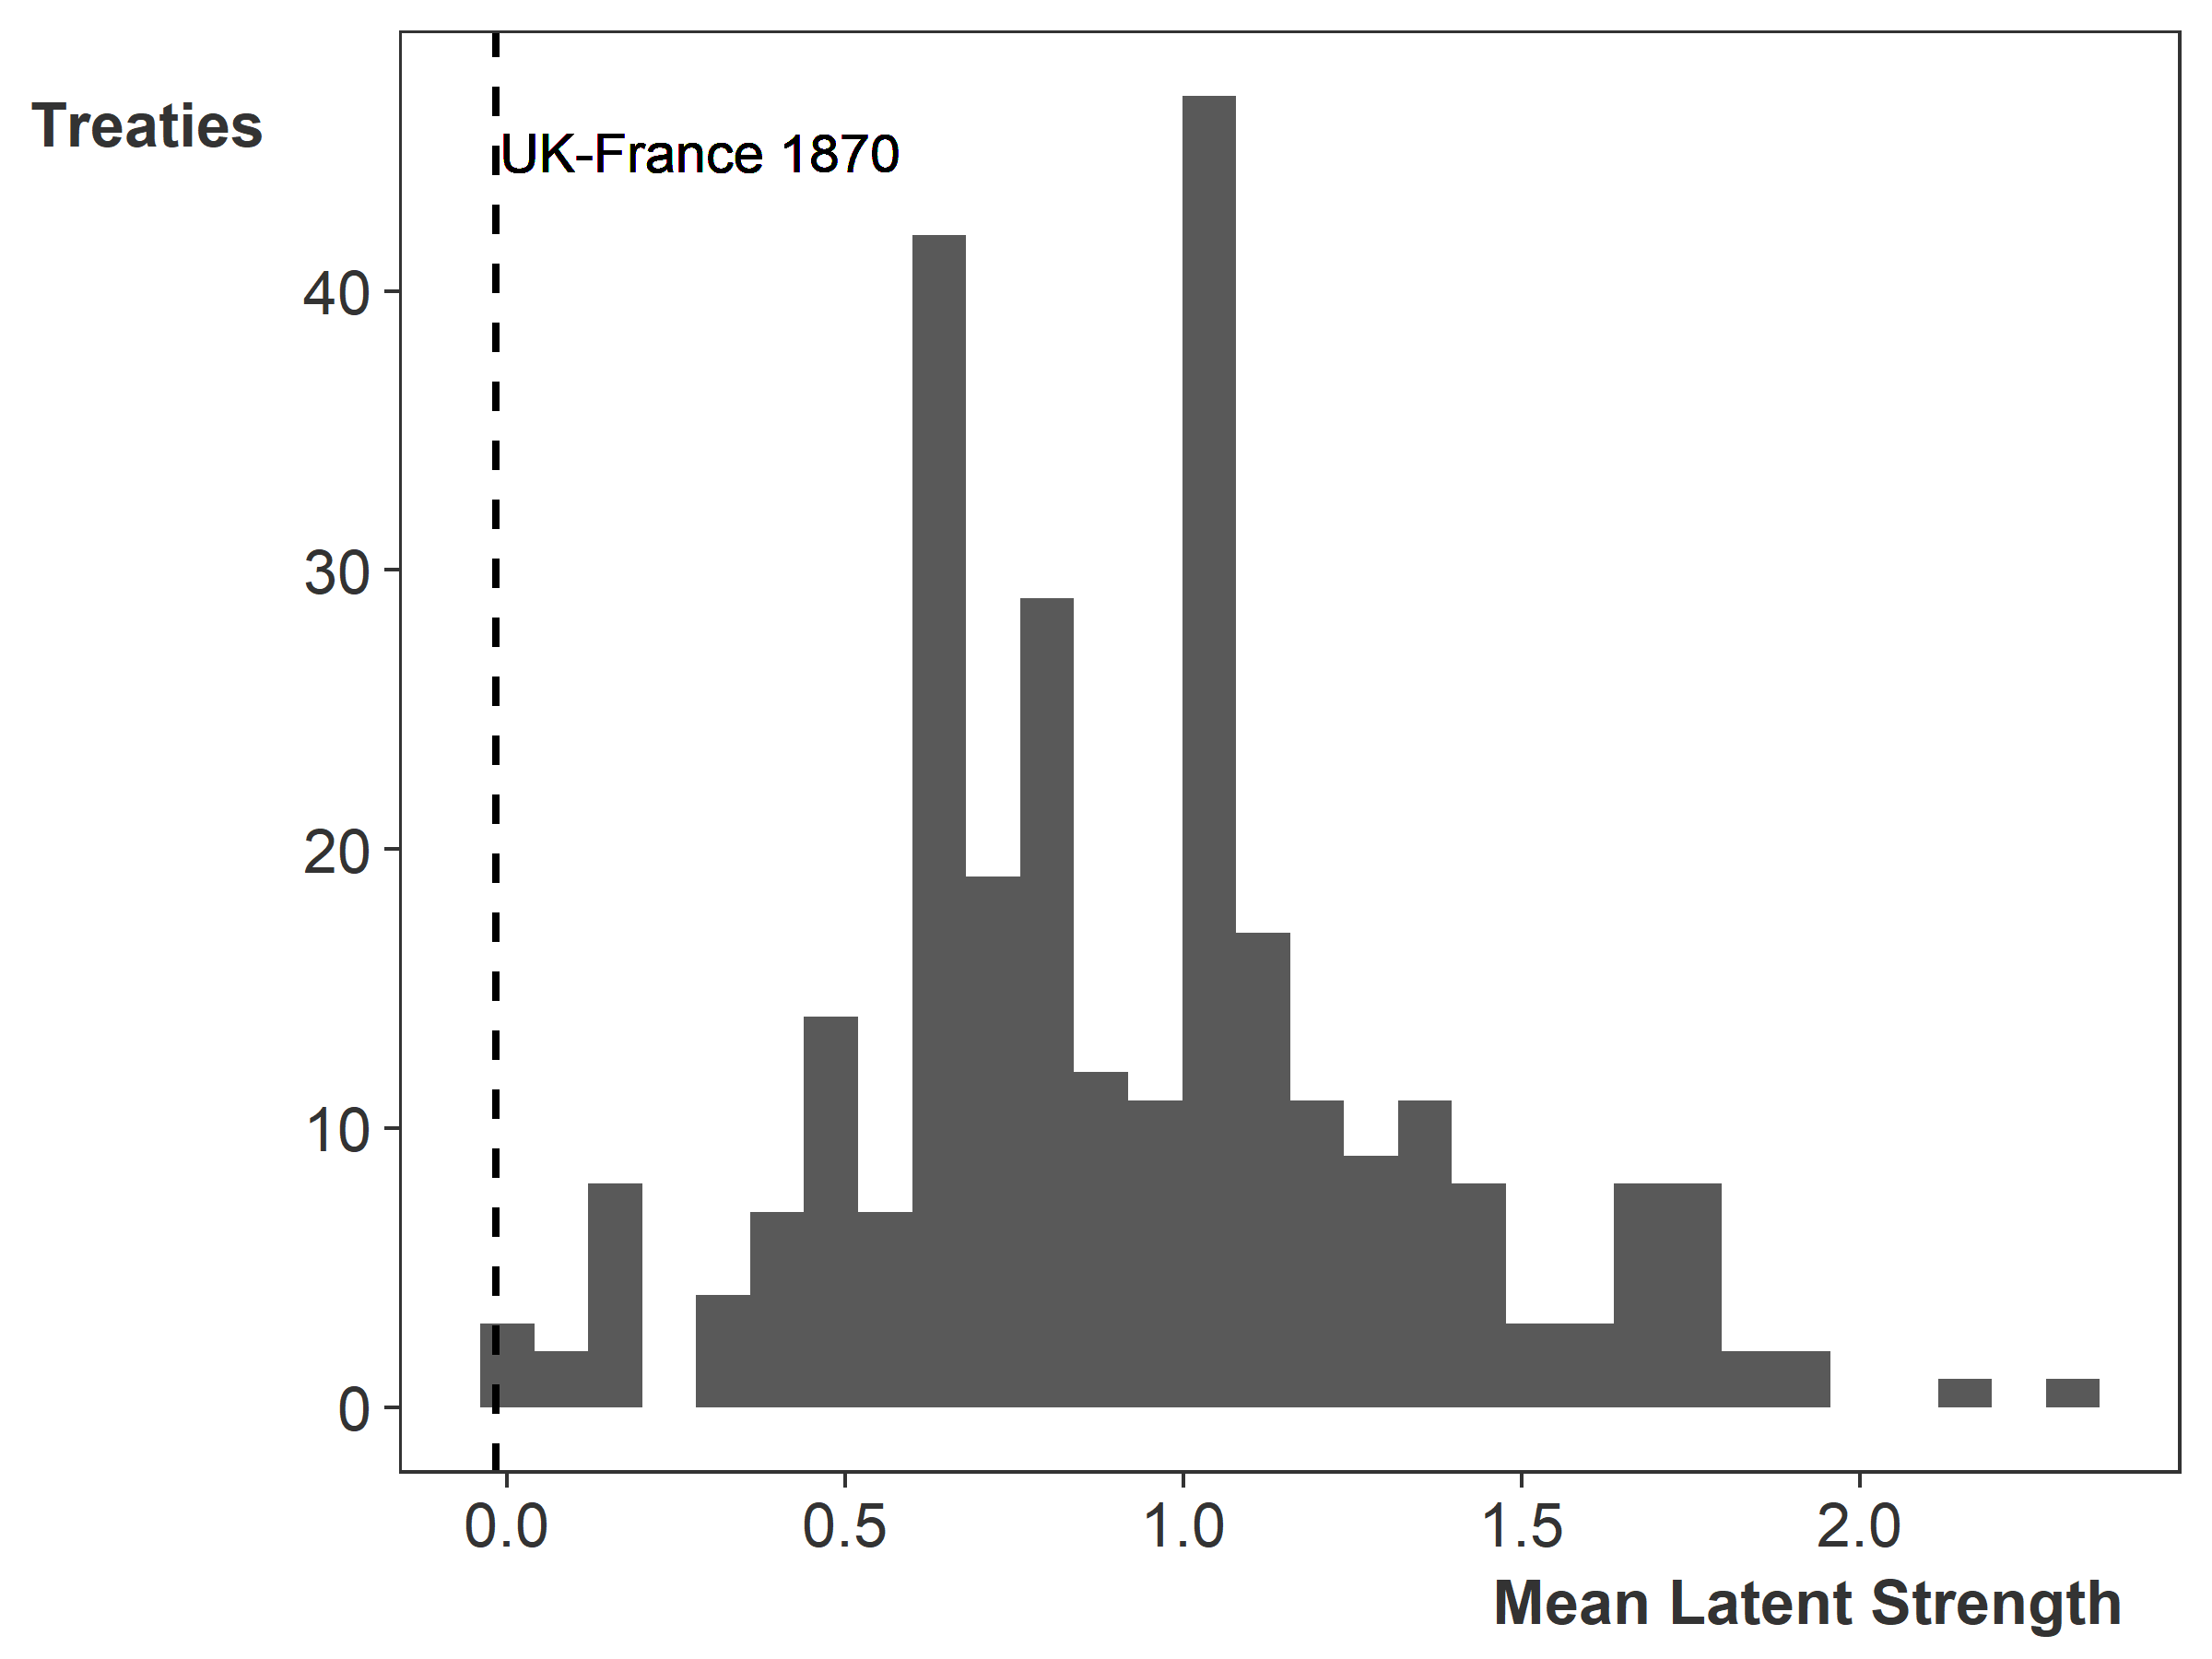
\includegraphics[width=0.95\textwidth]{ls-hist-weak.png}
\end{figure}


\end{frame} 

%------------------------------------------------

\begin{frame}{Latent Measure of Treaty Strength: Typical}

% Visual summary of latent measure
\begin{figure}[htbp]
	\centering
		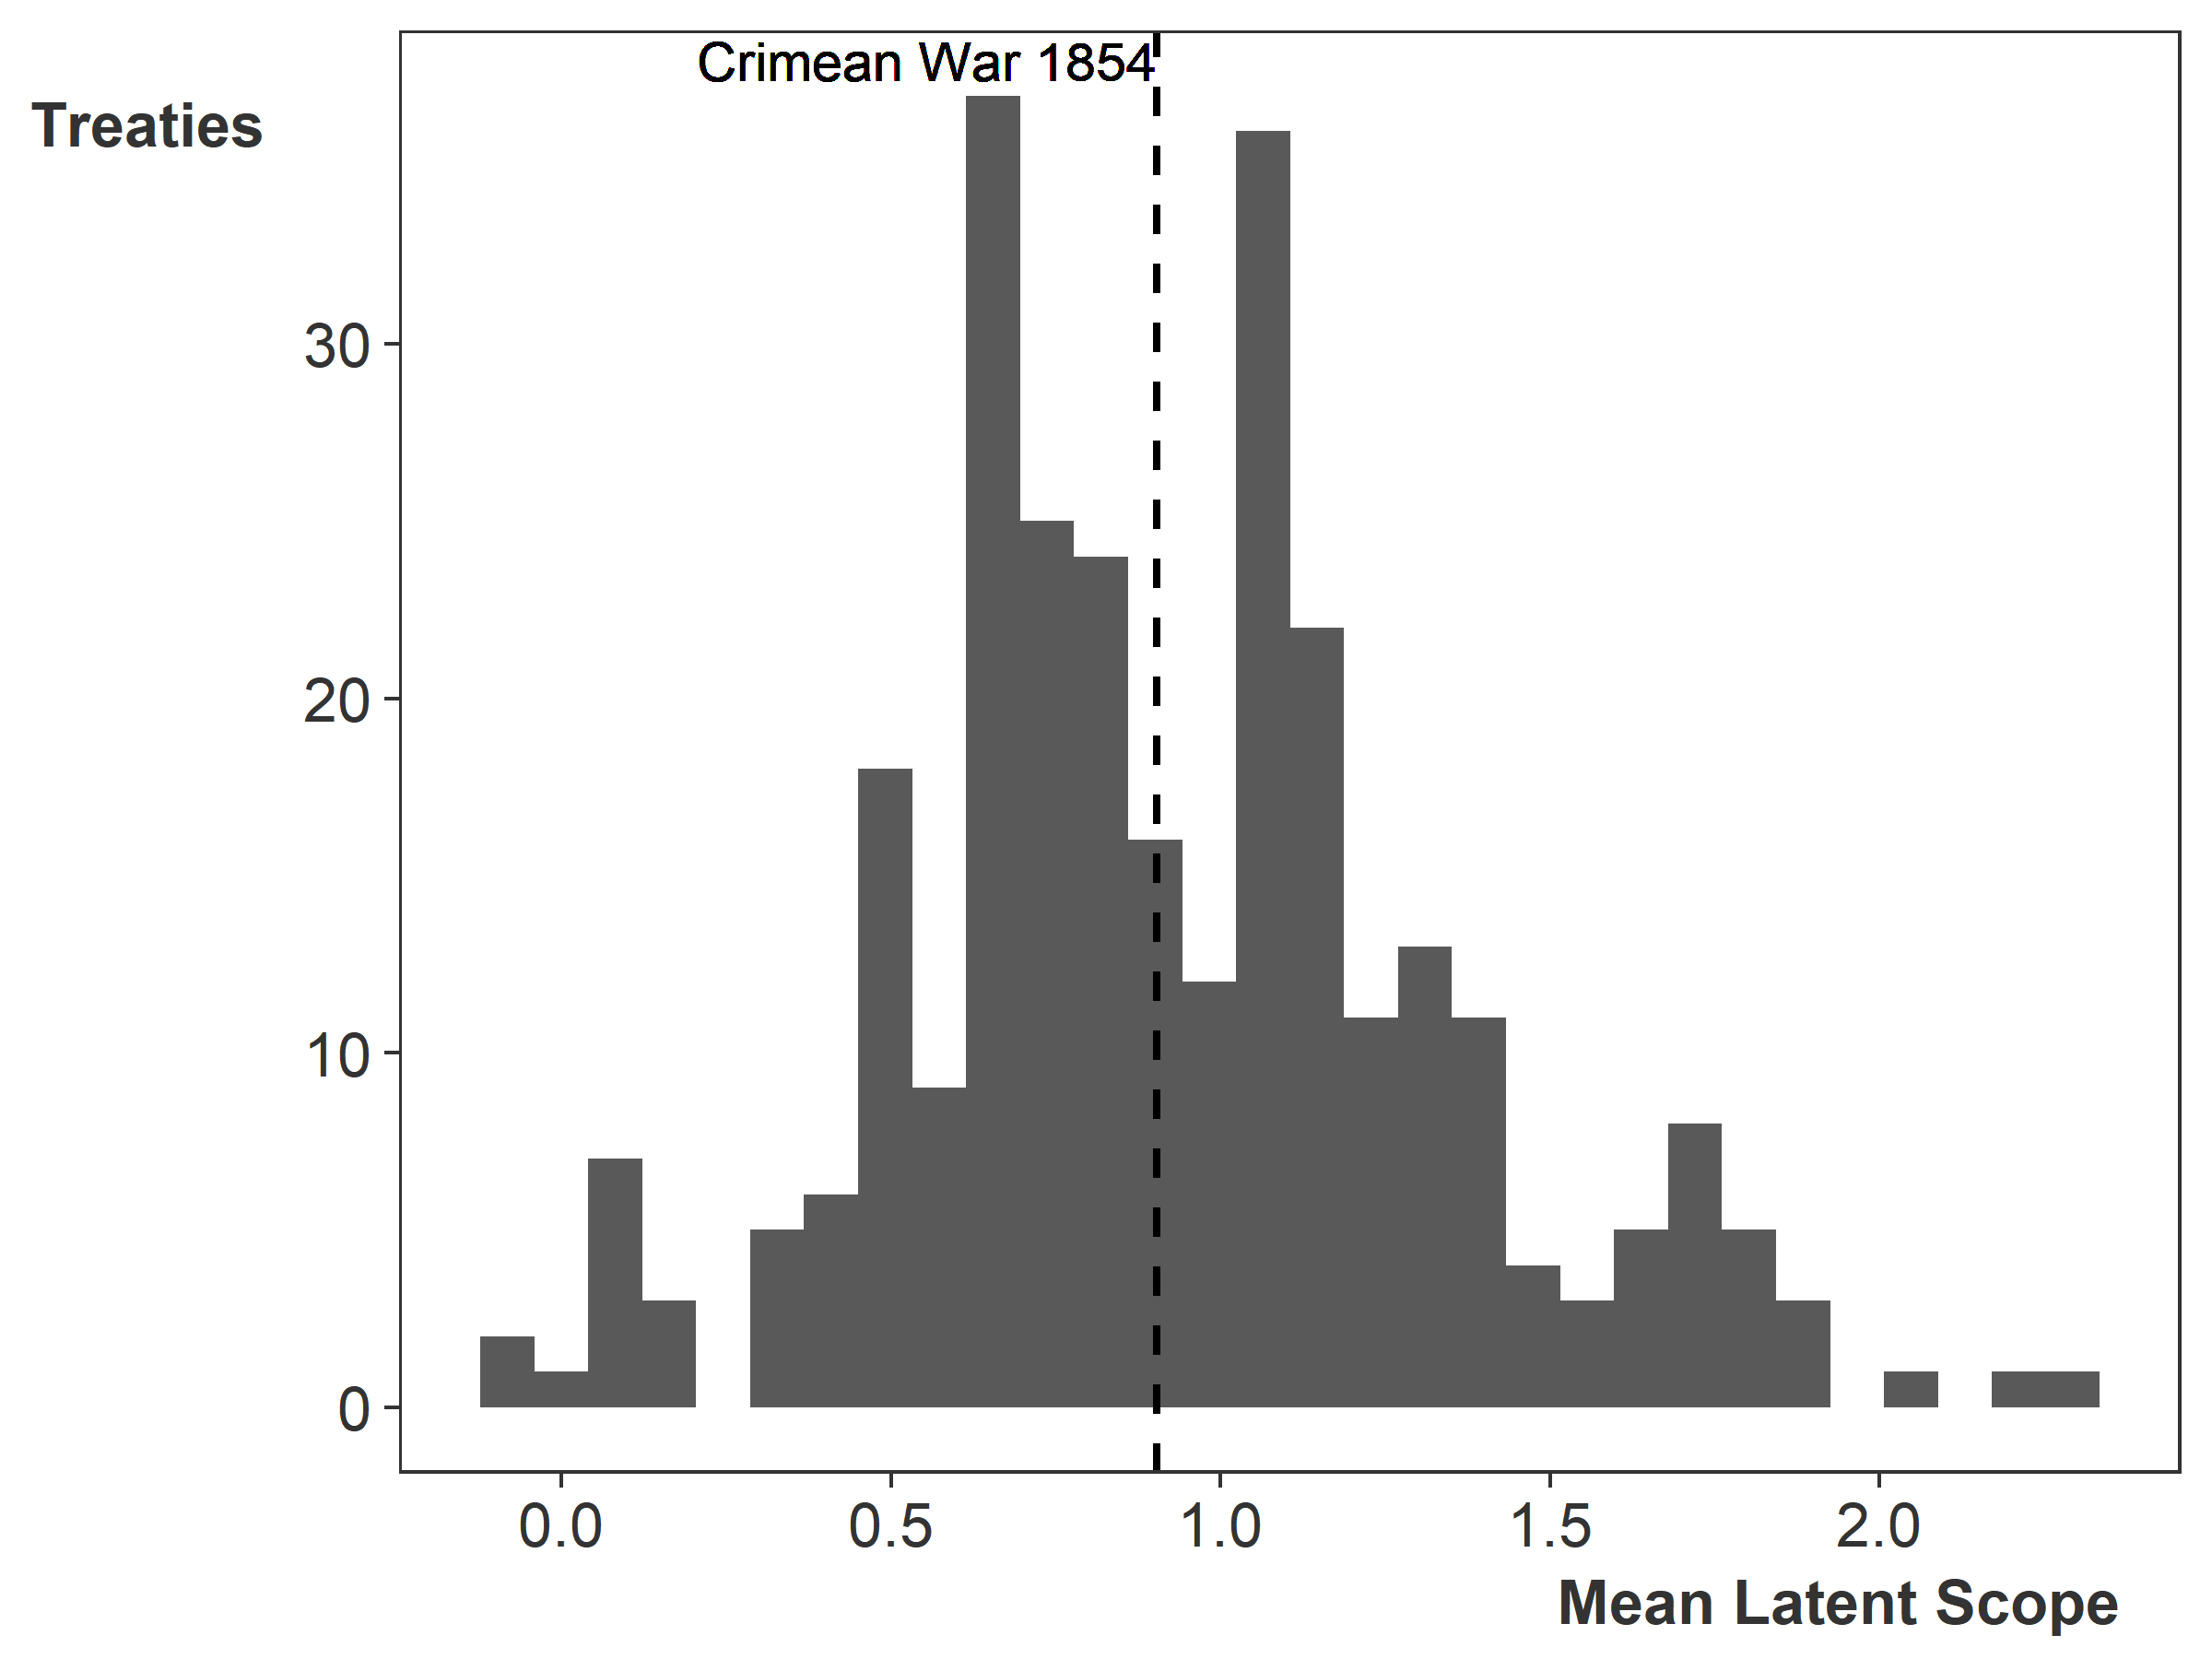
\includegraphics[width=0.95\textwidth]{ls-hist-median.png}
\end{figure}


\end{frame} 

%------------------------------------------------

\begin{frame}{Latent Measure of Treaty Strength: Strong}

% Visual summary of latent measure
\begin{figure}[htbp]
	\centering
		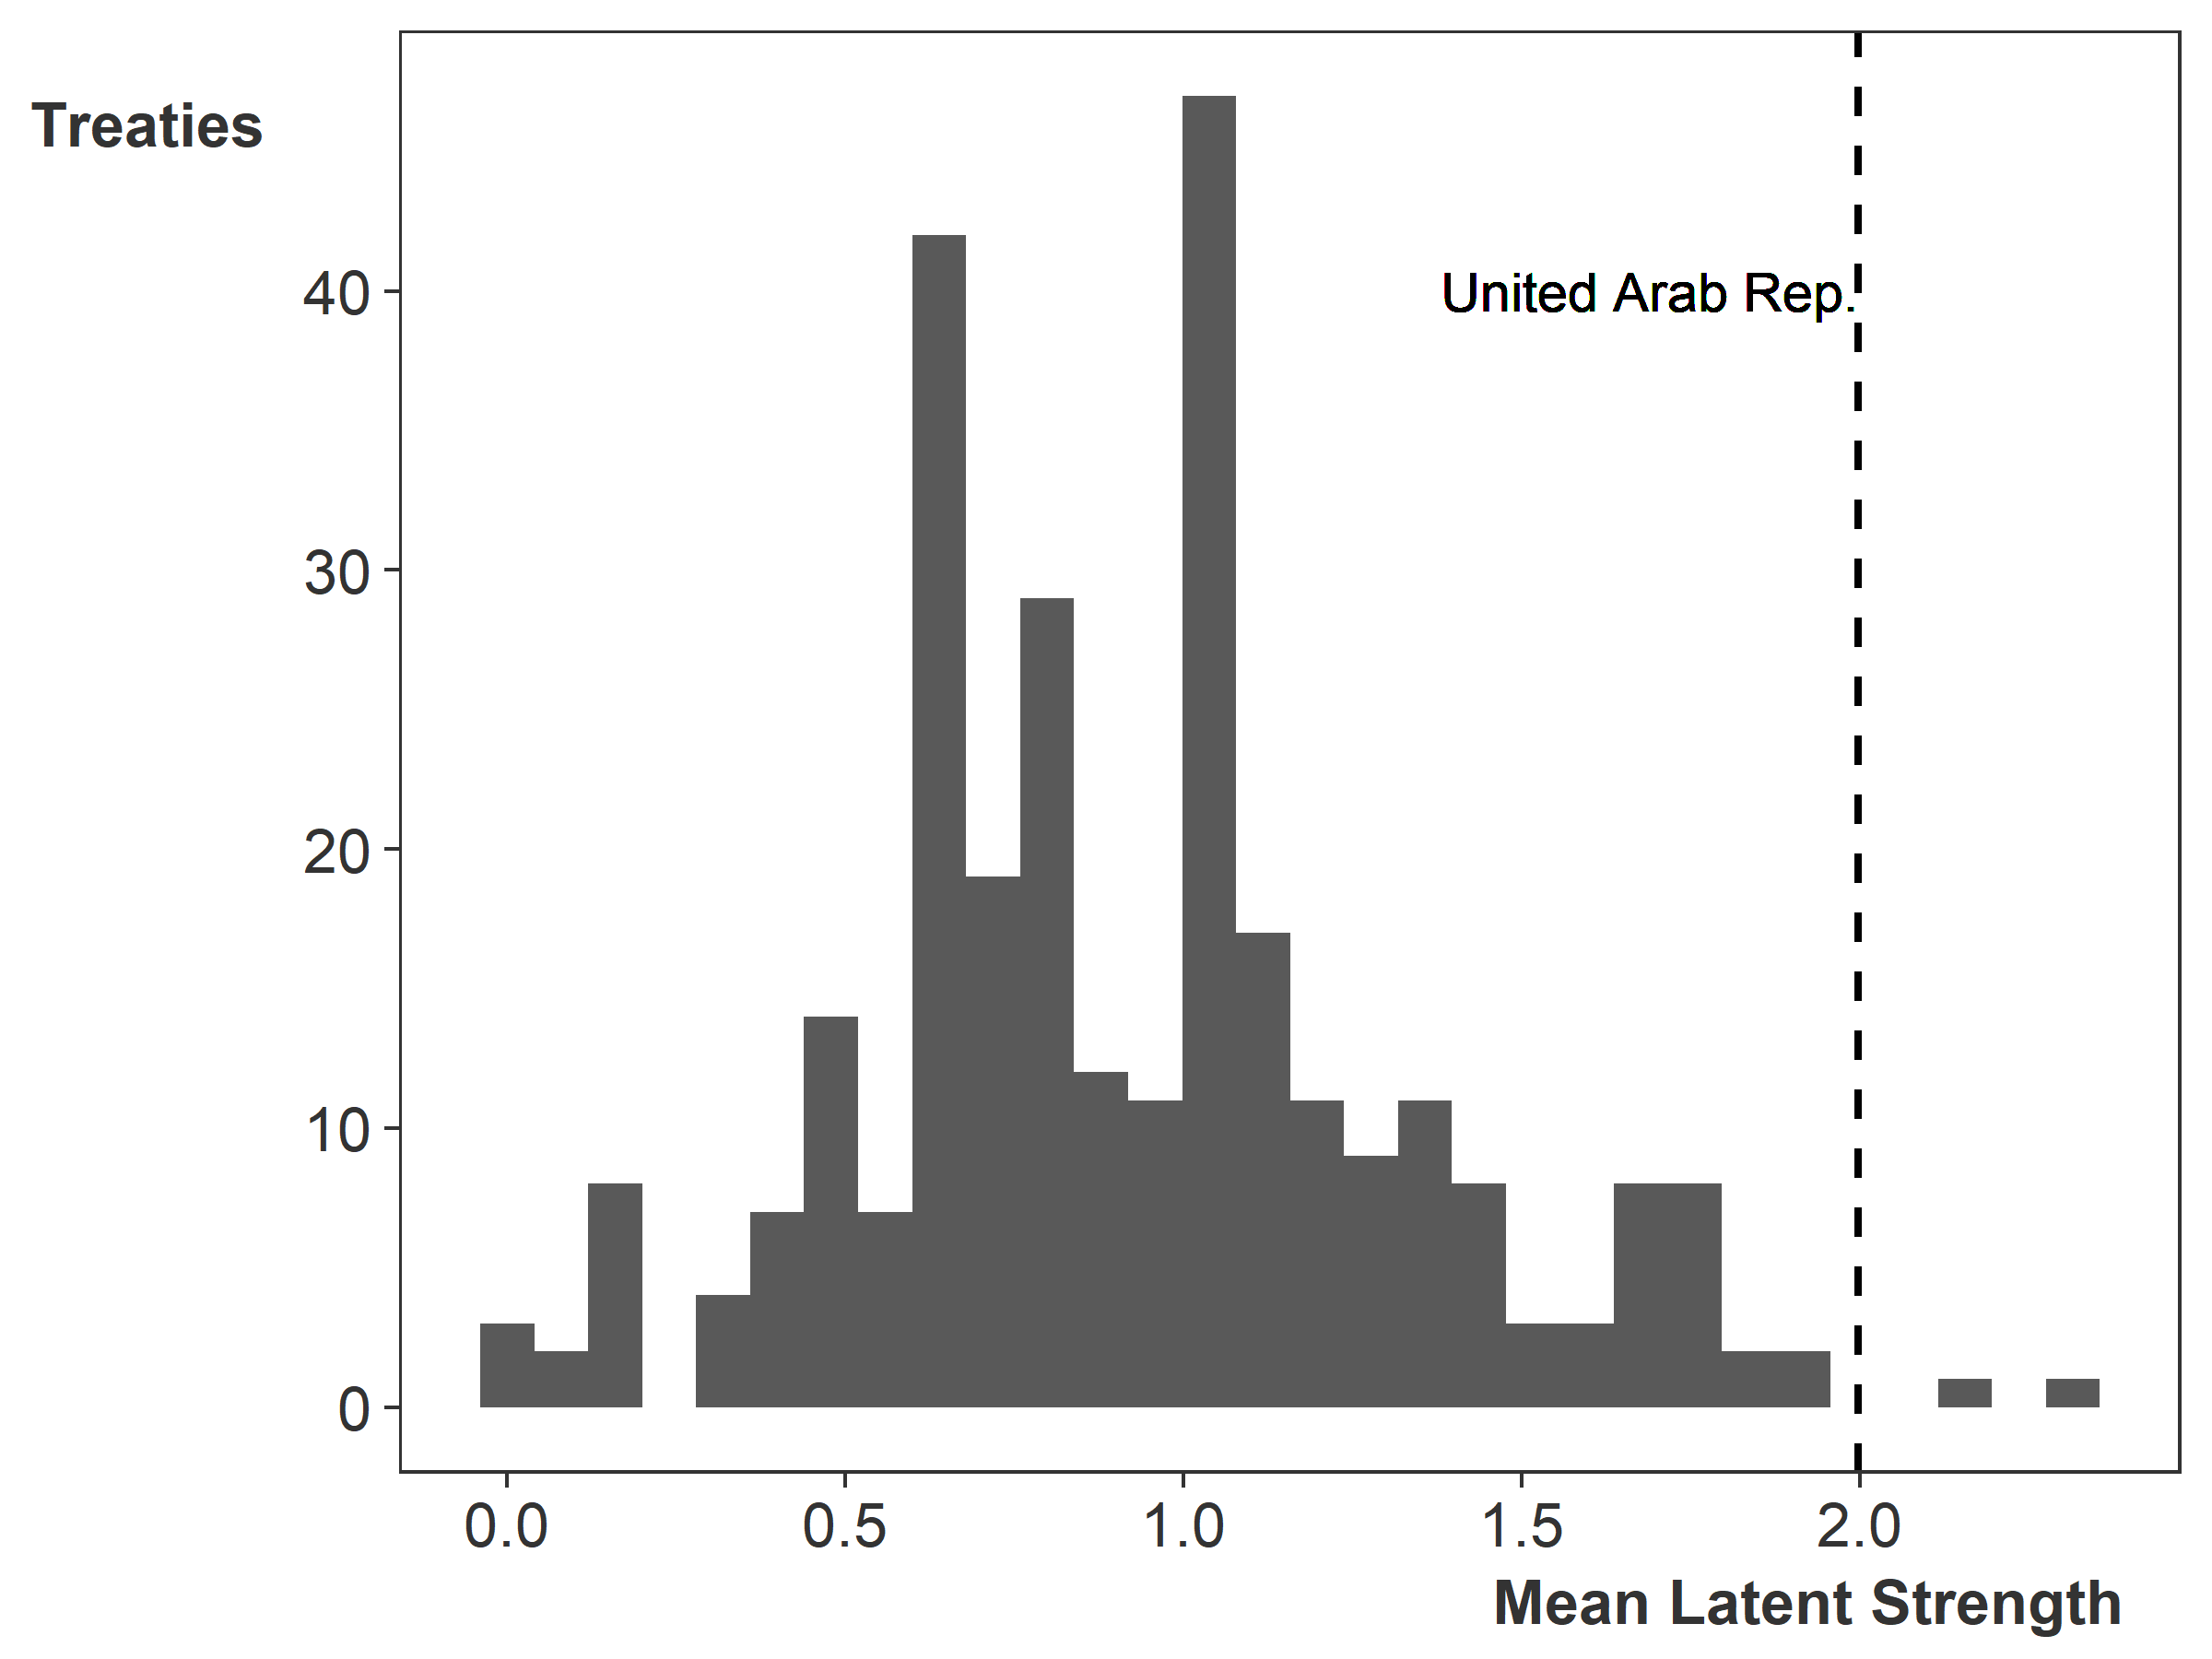
\includegraphics[width=0.95\textwidth]{ls-hist-strong.png}
\end{figure}


\end{frame} 

%------------------------------------------------


\begin{frame}{Single-Level Robust Regression}

\begin{figure}[htbp]
	\centering
		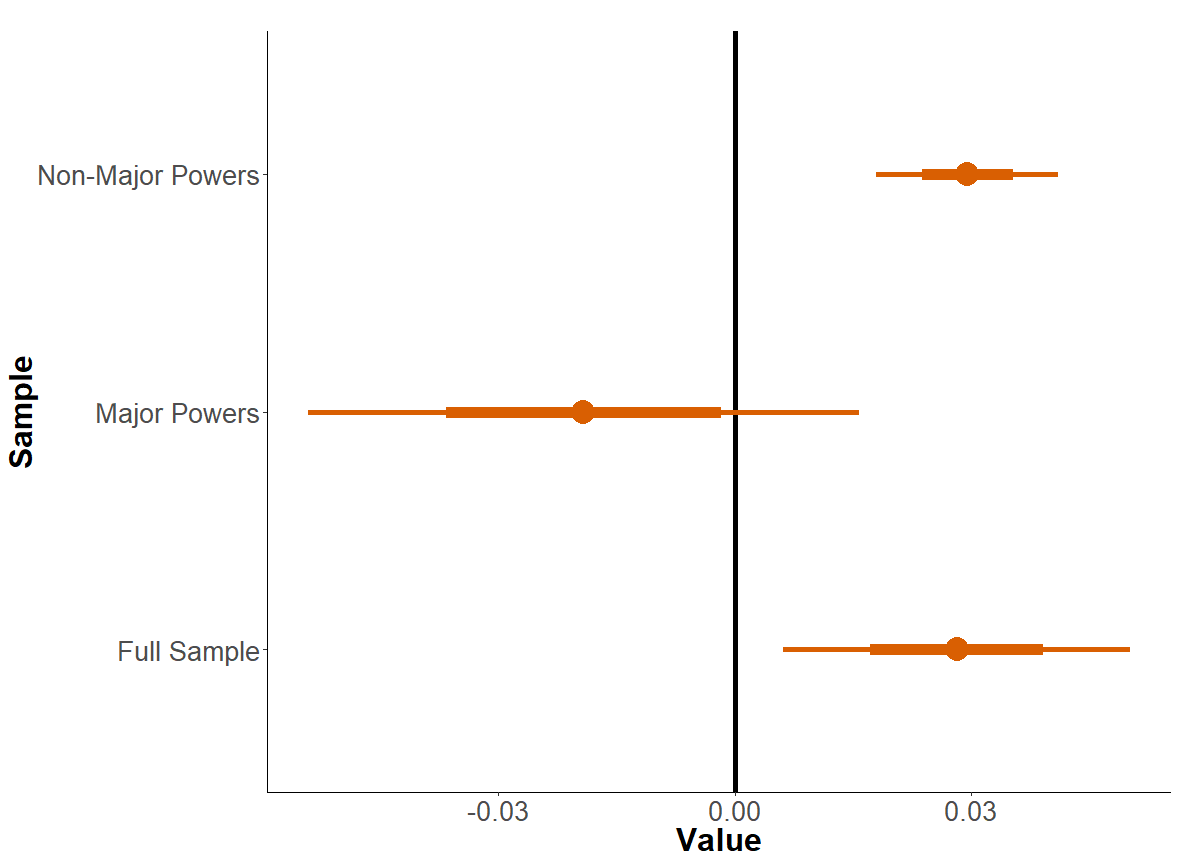
\includegraphics[width=0.95\textwidth]{robust-reg-coef.png}
	\label{fig:robust-reg-coef}
\end{figure}



\end{frame}



%----------------------------------------------------------------------------------------

\end{document}